\documentclass[10pt,twocolumn,letterpaper]{article}


\usepackage{xeCJK}


\usepackage{iccv}
\usepackage{times}
\usepackage{epsfig}
\usepackage{graphicx}
\usepackage{amsmath}
\usepackage{amssymb}

% Include other packages here, before hyperref.
%% \usepackage[accsupp]{axessibility}  % Improves PDF readability for those with disabilities.

\usepackage{booktabs}
\usepackage{hhline}

\usepackage{amssymb}% http://ctan.org/pkg/amssymb
\usepackage{pifont}% http://ctan.org/pkg/pifont
\newcommand{\cmark}{\ding{51}}%
\newcommand{\xmark}{\ding{55}}%

\usepackage[pagebackref=true,breaklinks=true,letterpaper=true,colorlinks,bookmarks=false]{hyperref}


% If you comment hyperref and then uncomment it, you should delete
% egpaper.aux before re-running latex.  (Or just hit 'q' on the first latex
% run, let it finish, and you should be clear).
%\usepackage[breaklinks=true,bookmarks=false]{hyperref}



\iccvfinalcopy % *** Uncomment this line for the final submission

\def\iccvPaperID{9187} % *** Enter the ICCV Paper ID here
\def\httilde{\mbox{\tt\raisebox{-.5ex}{\symbol{126}}}}

% Pages are numbered in submission mode, and unnumbered in camera-ready
\ificcvfinal\pagestyle{empty}\fi

\begin{document}

%%%%%%%%% TITLE
% \title{Pixel Difference Networks for Efficient Edge Detection}
\title{用于高效边缘检测的像素差分网络}


\author{Zhuo Su$^{1,\ast}$\;\;\;\;\;
Wenzhe Liu$^{2,}$\thanks{Equal contributions.\;\;\;$\dagger$ Corresponding author: \href{http://lilyliliu.com}{http://lilyliliu.com}}\;\;\;\;\;
Zitong Yu$^1$\;\;\;\;\;
Dewen Hu$^2$\;\;\;\;\;
Qing Liao$^3$\;\;\;\;\;
Qi Tian$^4$\\
Matti Pietik{\"a}inen$^1$\;\;\;\;\;
Li Liu$^{2,1,\dagger}$\\
$^1$Center for Machine Vision and Signal Analysis, University of Oulu, Finland\\
$^2$National University of Defense Technology, China\\
$^3$Harbin Institute of Technology (Shenzhen), China\;\;\;\;\;$^4$Xidian University, China\\
{\tt\small \{zhuo.su, zitong.yu, matti.pietikainen, li.liu\}@oulu.fi}\\ 
{\tt\small \{liuwenzhe15, dwhu\}@nudt.edu.cn, liaoqing@hit.edu.cn, wywqtian@gmail.com}
}




\maketitle
% Remove page # from the first page of camera-ready.
\ificcvfinal\thispagestyle{empty}\fi

%%%%%%%%% ABSTRACT
\begin{abstract}
% Recently, deep Convolutional Neural Networks (CNNs) can achieve human-level performance in edge detection with the rich and abstract edge representation capacities. However, the high performance of CNN based edge detection is achieved with a large pretrained CNN backbone, which is memory and energy consuming. In addition, it is surprising that the previous wisdom from the traditional edge detectors, such as Canny, Sobel, and LBP are rarely investigated in the rapid-developing deep learning era. To address these issues, we propose a simple, lightweight yet effective architecture named Pixel Difference Network (PiDiNet) for efficient edge detection. PiDiNet adopts novel pixel difference convolutions that integrate the traditional edge detection operators into the popular convolutional operations in modern CNNs for enhanced performance on the task, which enjoys the best of both worlds. Extensive experiments on BSDS500, NYUD, and Multicue are provided to demonstrate its effectiveness, and its high training and inference efficiency. Surprisingly, when training from scratch with only the BSDS500 and VOC datasets, PiDiNet can surpass the recorded result of human perception (0.807 vs. 0.803 in ODS F-measure) on the BSDS500 dataset with 100 FPS and less than 1M parameters. A faster version of PiDiNet with less than 0.1M parameters can still achieve comparable performance among state of the arts with 200 FPS. Results on the NYUD and Multicue datasets show similar observations. The codes are available at  \href{https://github.com/zhuoinoulu/pidinet}{https://github.com/zhuoinoulu/pidinet}.

近年来,深度卷积神经网络(CNN)以其丰富而抽象的边缘表示能力,在边缘检测方面取得了人类水平的性能。然而,基于CNN的边缘检测的高性能是通过大型预训练的CNN主干实现的,这会大量消耗内存和能量。此外,令人惊讶的是,在快速发展的深度学习时代,传统边缘检测器(如Canny、Sobel和LBP)的智慧很少被研究。为了解决这些问题,我们提出了一种简单、轻量级但有效的架构,称为像素差分网络(PiDiNet),用于高效的边缘检测。PiDiNet采用新颖的像素差分卷积,将传统的边缘检测算子集成到现代CNN中流行的卷积运算中,以增强任务性能,两全其美。提供了在BSDS500、NYUD和Multicue上的大量实验,以证明其有效性以及高训练和推理效率。令人惊讶的是,当仅使用BSDS500和VOC数据集从头开始训练时,PiDiNet可以在100 FPS和小于1M的参数的BSDS500数据集上超过人类感知的记录结果(0.807 vs. ODS F-measure中的0.803)。参数少于0.1M的更快版本的PiDiNet仍然可以在具有200 FPS的最新技术中实现可比的性能。NYUD和Multicue数据集的结果显示了类似的观察结果。代码可在\href{https://github.com/zhuoinoulu/pidinet}{https://github.com/zhuoinoulu/pidinet}获取。
\end{abstract}

%%%%%%%%% BODY TEXT
% \section{Introduction}
\section{简介}
\label{sec:intro}


% Edge detection has been a longstanding, fundamental low-level problem in computer vision~\cite{canny1986computational}. Edges and object boundaries play an important role in various higher-level computer vision tasks such as object recognition and detection \cite{liu2020deep,ferrari2007groups}, object proposal generation \cite{cheng2014bing,uijlings2013selective}, image editing \cite{elder1998imageediting}, and image segmentation \cite{muthukrishnan2011edgeimageseg,bertasius2016semantic}. Therefore, recently, the edge detection problem has also been revisited and injected new vitality due to the renaissance of deep learning~\cite{bertasius2015deepedge,kokkinos2015deepboundary,shen2015deepcontour,xie2017holistically,wang2017ced,liu2019richer}.
边缘检测一直是计算机视觉中一个长期存在的基本低层级问题~\cite{canny1986computational}。边缘和对象边界在各种更高级别的计算机视觉任务中起着重要作用,例如对象识别和检测~\cite{liu2020deep, ferrari2007groups}、对象提议生成~\cite{cheng2014bing, uijlings2013selective}、图像编辑~\cite{elder1998imageediting}和图像分割~\cite{muthukrishnan2011edgeimageseg, bertasius2016semantic}。因此,最近由于深度学习的复兴,边缘检测问题也被重新审视并注入了新的活力~\cite{bertasius2015deepedge, kokkinos2015deepboundary, shen2015deepcontour, xie2017holistically, wang2017ced, liu2019richer}。


\begin{figure}[t!]
    \centering
    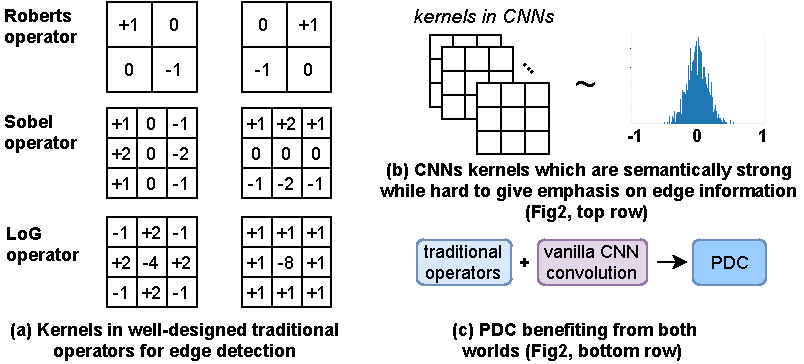
\includegraphics[width=0.98\linewidth]{images/fig1_rebuttal.pdf}
    % \caption{PDC benefits from both worlds with proper integration of traditional operators and modern CNNs.}
    \caption{PDC通过传统算子和现代CNN的适当集成,从这两个方面受益。}
    \label{fig:figure1}
\end{figure}

\begin{figure*}[t!]
    \centering
    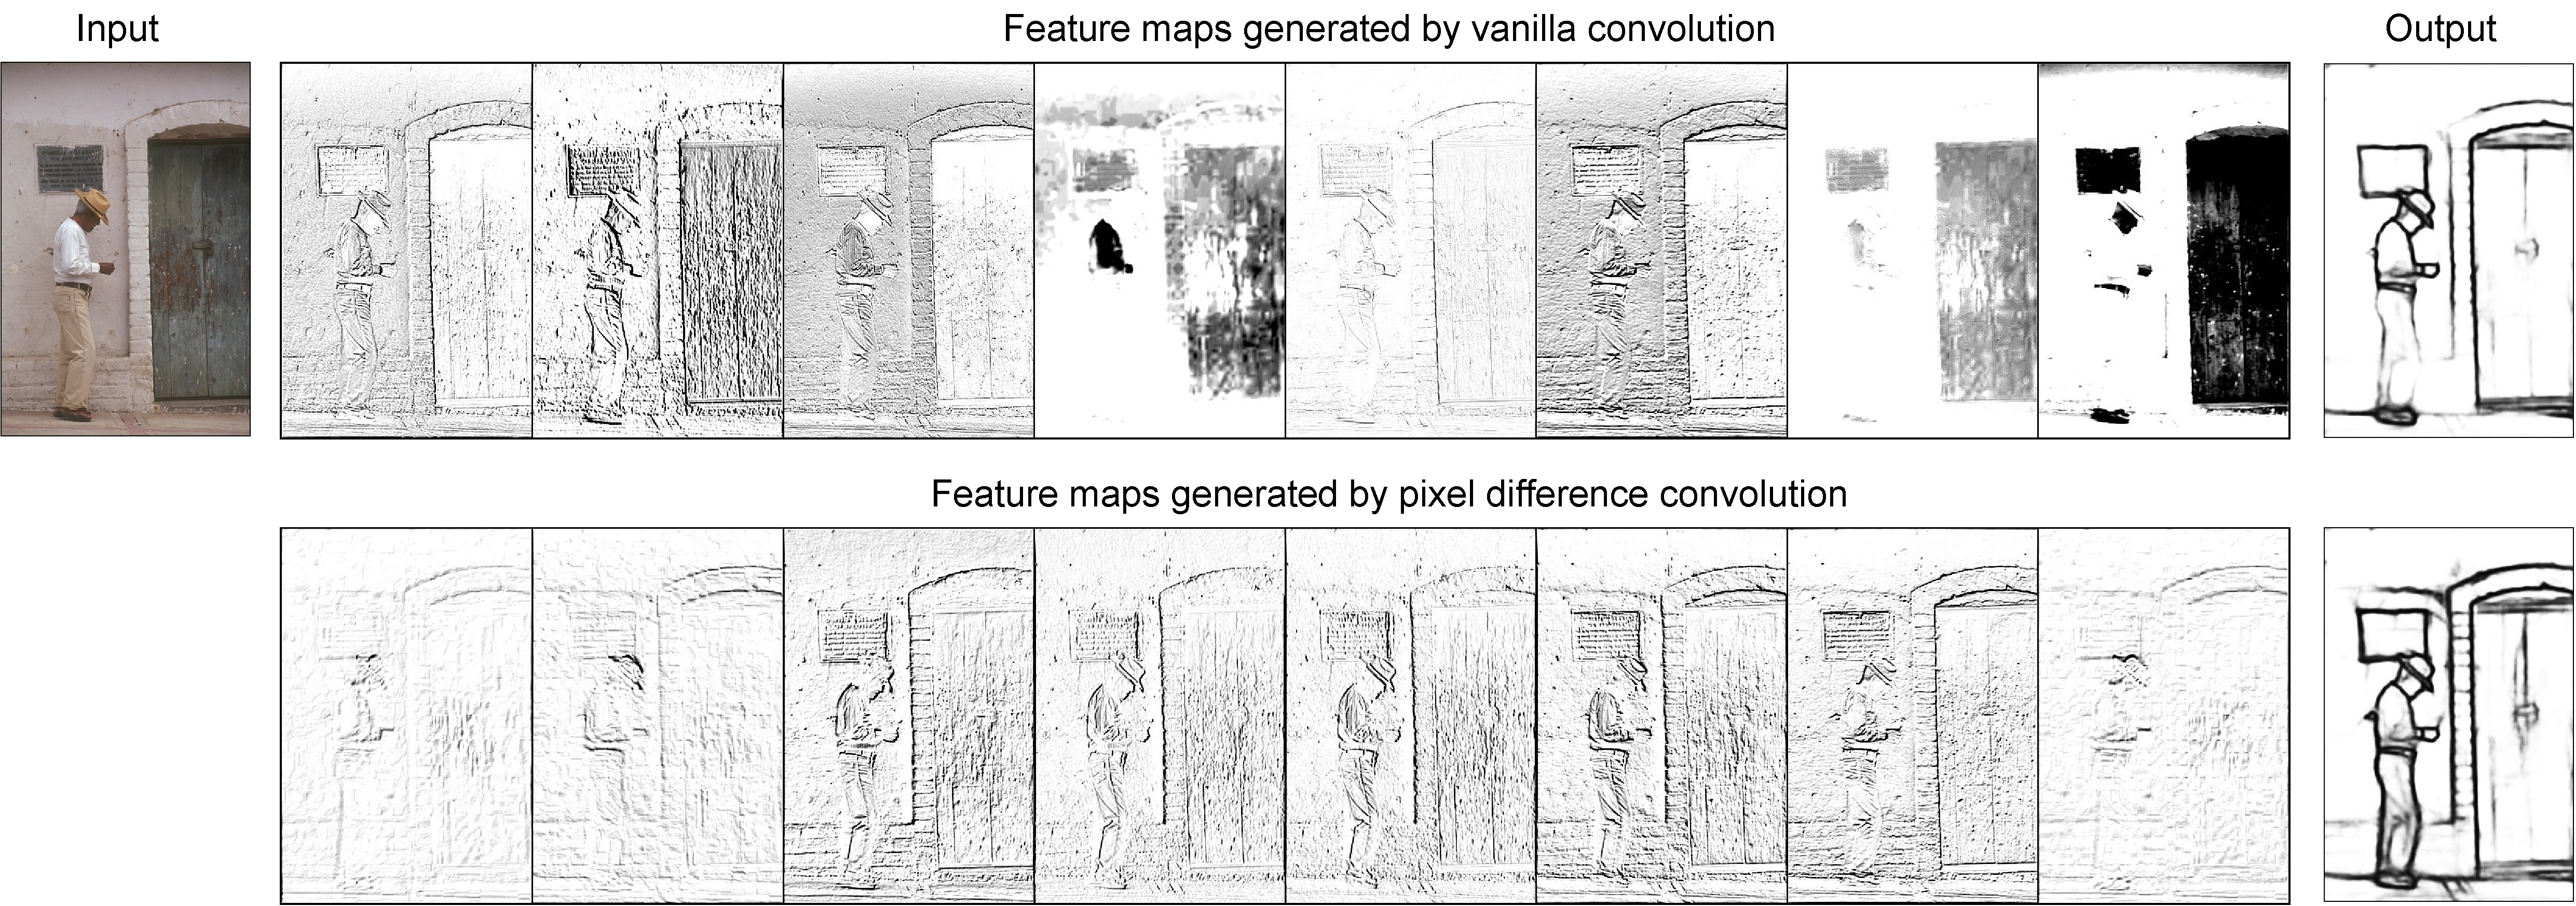
\includegraphics[width=0.98\linewidth]{images/figure_intro2.pdf}
    % \caption{PiDiNet configured with pixel difference convolution (PDC) \emph{vs.} the baseline with vanilla convolution. Both models were trained only using the BSDS500 dataset. Compared with vanilla convolution, PDC can better capture gradient information from the image that facilitates edge detection.}
    \caption{配置了像素差异卷积(PDC)的PiDiNet\emph{对比}带有普通卷积的基线。两种模型都仅使用BSDS500数据集进行训练。与普通卷积相比,PDC可以更好地从图像中捕获梯度信息,便于边缘检测。}
    \label{fig:figure2}
\end{figure*}


% The main goal of edge detection is identifying sharp image brightness changes such as discontinuities in intensity, color, or texture~\cite{torre1986edge}. Traditionally, edge detectors based on image gradients or derivatives information are popular choices. Early classical methods use the first or second order derivatives (\emph{e.g.}, Sobel~\cite{sobel19683x3}, Prewitt~\cite{prewitt1970object}, Laplacian of Gaussian (LoG), Canny~\cite{canny1986computational}, \emph{etc.}) for basic edge detection. Later learning based methods~\cite{hallman2015oef,dollar2014se} further utilize various gradient information~\cite{xiaofeng2012scg, martin2004pb,fowlkes2002learningpb,gupta2014seng} to produce more accurate boundaries.
边缘检测的主要目标是识别锐利的图像亮度变化,例如强度、颜色或纹理的不连续性~\cite{torre1986edge}。传统上,基于图像梯度或导数信息的边缘检测器是流行的选择。早期的经典方法使用一阶或二阶导数(\emph{例如}:Sobel~\cite{sobel19683x3}、Prewitt~\cite{prewitt1970object}、Laplacian of Gaussian(LoG)、Canny~\cite{canny1986computational}\emph{等等})用于基本边缘检测。基于后期学习的方法~\cite{hallman2015oef, dollar2014se}进一步利用各种梯度信息~\cite{xiaofeng2012scg, martin2004pb, fowlkes2002learningpb, gupta2014seng}产生更准确的边界。

% Due to the capability of automatically learning rich representations of data with hierarchical levels of abstraction, deep CNNs have brought tremendous progress for various computer vision tasks including edge detection and are still rapidly developing. Early deep learning based edge detection models construct CNN architectures as classifiers to predict the edge probability of an input image patch~\cite{bertasius2015deepedge,shen2015deepcontour,bertasius2015hfl}. Building on top of fully convolutional networks~\cite{long2015fully}, HED~\cite{xie2017holistically} performs end-to-end edge detection by leveraging multilevel image features with rich hierarchical information guided by deep supervision, and achieves state-of-the-art performance. Other similar works include~\cite{yang2016cedn,kokkinos2015deepboundary,maninis2016cob,wang2017ced,xu2018amhnet,liu2019richer,deng2018lpcb,he2019bidirectional}.
由于能够自动学习具有分层抽象层次的数据的丰富表示,深度CNN为包括边缘检测在内的各种计算机视觉任务带来了巨大的进步,并且仍在快速发展。早期基于深度学习的边缘检测模型构建CNN架构作为分类器来预测输入图像块的边缘概率~\cite{bertasius2015deepedge, shen2015deepcontour, bertasius2015hfl}。建立在全卷积网络~\cite{long2015fully}之上,HED~\cite{xie2017holistically}通过利用深度监督指导下的具有丰富层次信息的多级图像特征来执行端到端边缘检测,并实现最先进的性能。其他类似的工作还有~\cite{yang2016cedn, kokkinos2015deepboundary, maninis2016cob, wang2017ced, xu2018amhnet, liu2019richer, deng2018lpcb, he2019bidirectional}。

% However, integration of traditional edge detectors with modern CNNs were rarely investigated. The former were merely utilized as auxiliary tools to extract candidate edge points in some prior approaches~\cite{bertasius2015hfl,bertasius2015deepedge}. Intuitively, edges manifest diverse specific patterns like straight lines, corners, and ``X'' junctions. On one hand, traditional edge operators like those shown in Fig. 1 are inspired by these intuitions, and based on gradient computing which encodes important gradient information for edge detection by explicitly calculating pixel differences. However, these handcrafted edge operators or learning based edge detection algorithms are usually not powerful enough due to their shallow structures. On the other hand, modern CNNs can learn rich and hierarchical image representations, where vanilla CNN kernels serve as probing local image patterns. Nevertheless, CNN kernels are optimized by starting from random initialization which has no explicit encoding for gradient information, making them hard to focus on edge related features.
然而,将传统边缘检测器与现代CNN相结合的研究很少。前者在一些先前的方法中仅用作提取候选边缘点的辅助工具~\cite{bertasius2015hfl, bertasius2015deepedge}。直观地,边缘表现出不同的特定模式,如直线、角和“X”连接。一方面,像Fig. \ref{fig:figure1}所示的传统边缘算子受到这些直觉的启发,并基于梯度计算,通过显式计算像素差异来编码边缘检测的重要梯度信息。然而,这些手工制作的边缘算子或基于学习的边缘检测算法由于其浅层结构通常不够强大。另一方面,现代CNN可以学习丰富的分层图像表示,其中普通CNN卷积核用作探测局部图像模式。然而,CNN卷积核是通过从随机初始化开始优化的,它没有对梯度信息进行显式编码,这使得它们很难专注于边缘相关的特征。


\begin{table}[t!]
% \caption{Comparison between ours and some leading edge detection models in terms of efficiency and accuracy. The multiply-accumulates (MACs) are calculated based on a 200$\times$200 image, FPS and ODS \emph{F-measure} are evaluated on the BSDS500 test set.}
\caption{在效率和准确性方面,我们与一些领先的边缘检测模型进行了比较。乘法累加(MACs)是基于200$ \times $200图像计算的,FPS和ODS \emph{F-measure}在BSDS500测试集上进行评估。}
\begin{center}
\setlength{\tabcolsep}{0.015\linewidth}
\resizebox*{\linewidth}{!}{
\begin{tabular}{lccccc}
\toprule[1pt]
 & \emph{HED}~\cite{xie2017holistically} & \emph{RCF}~\cite{liu2019richer} & \emph{BDCN}~\cite{he2019bidirectional} & \emph{PiDiNet} & \emph{PiDiNet(tiny)} \\
\hline
Params & 14.7M & 14.8M & 16.3M & 710K & 73K \\
MACs & 22.2G & 16.2G & 23.2G & 3.43G & 270M \\
Throughput & 78FPS & 67FPS & 47FPS & 92FPS & 215FPS\\
Pre-training & ImageNet & ImageNet & ImageNet & No & No \\
ODS \emph{F-measure} & 0.788 & 0.806 & 0.820 & 0.807 & 0.787 \\
\bottomrule[1pt]
\end{tabular}
}
\end{center}
\label{table:table1}
\vspace{-0.2in}
\end{table}

% We believe a new type of convolutional operation can be derived, to satisfy the following needs. Firstly, it can easily capture the image gradient information that facilitates edge detection, and the CNN model can be more focused with the release of burden on dealing with much unrelated image features. Secondly, the powerful learning ability of deep CNNs can still be preserved, to extract semantically meaningful representations, which lead to robust and accurate edge detection. In this paper, we propose pixel difference convolution (PDC), where the pixel differences in the image are firstly computed, and then convolved with the kernel weights to generate output features (see Fig.~\ref{fig:pdc}). We show PDC can effectively improve the quality of the output edge maps, as illustrated in Fig.~\ref{fig:figure2}.
我们相信可以推导出一种新型的卷积运算,以满足以下需求。首先,它可以轻松捕获有利于边缘检测的图像梯度信息,并且CNN模型可以更加专注于处理许多不相关的图像特征的负担。其次,仍然可以保留深度CNN的强大学习能力,以提取具有语义意义的表示,从而实现稳健而准确的边缘检测。在本文中,我们提出了像素差分卷积(PDC),其中首先计算图像中的像素差分,然后与卷积核权重卷积以生成输出特征(见Fig. ~\ref{fig:pdc})。我们展示了PDC可以有效提高输出边缘图的质量,如Fig. ~\ref{fig:figure2}所示。

% On the other hand, leading CNN based edge detectors suffer from the deficiencies as shown in Table~\ref{table:table1}: being memory consuming with big model size, being energy hungry with high computational cost, running inefficiency with low throughput and label inefficiency with the need of model pre-training on large scale dataset. This is due to the fact that the annotated data available for training edge detection models is limited, and thus a well pretrained (usually large) backbone is needed. For example, the widely adopted routine is to use the large VGG16~\cite{simonyan2014very} architecture that was trained on the large scale ImageNet dataset~\cite{deng2009imagenet}.
另一方面,领先的基于CNN的边缘检测器存在以下缺陷,如Table ~\ref{table:table1}所示:模型尺寸大,内存消耗大,计算成本高,能耗高,运行效率低,吞吐量和标签效率低,需要在大规模数据集上进行模型预训练。这是因为可用于训练边缘检测模型的注释数据是有限的,因此需要一个经过良好预训练(通常很大)的主干。例如,广泛采用的例程是使用大型VGG16~\cite{simonyan2014very}架构,该架构在大规模ImageNet数据集~\cite{deng2009imagenet}上训练。

% It is important to develop a lightweight structure, to achieve a better trade-off between accuracy and efficiency for edge detection. With pixel difference convolution, inspired by~\cite{he2016residual,howard2017mobilenets}, we build a new end-to-end architecture, namely Pixel Difference Network (PiDiNet) to solve the mentioned issues in one time. Specifically, PiDiNet consists of an efficient backbone and an efficient task-specific side structure (see Fig.~\ref{fig:arch}), able to do robust and accurate edge detection with high efficiency.
开发轻量级结构以在边缘检测的准确性和效率之间实现更好的权衡非常重要。通过像素差分卷积,受~\cite{he2016residual, howard2017mobilenets}的启发,我们构建了一种新的端到端架构,即像素差分网络(PiDiNet)以一次性解决上述问题。具体来说,PiDiNet由一个高效的主干和一个高效的特定任务侧结构组成(见Fig. ~\ref{fig:arch}),能够高效地进行稳健而准确的边缘检测。


% \section{Related Work}
\section{相关工作}


% \noindent \textbf{Using Traditional Edge Detectors to Help Deep CNN Models for Edge Detection.} \quad Canny~\cite{canny1986computational} and SE~\cite{dollar2014se} edge detectors are usually used to extract candidate contour points before applying the CNN model for contour/non-contour prediction~\cite{bertasius2015deepedge, bertasius2015hfl}. The candidate points can be also used as auxiliary relaxed labels for better training the CNN model~\cite{liu2016relaxed}. Instead of relying on the edge information from the hand-crafted detectors, PDC directly integrates the gradient information extraction process into the convolutional operation, which is more compact and learnable.
\noindent \textbf{使用传统边缘检测器帮助深度CNN模型进行边缘检测。} \quad Canny~\cite{canny1986computational}和SE~\cite{dollar2014se}边缘检测器通常用于在应用CNN模型进行轮廓/非轮廓预测之前提取候选轮廓点~\cite{bertasius2015deepedge, bertasius2015hfl}。候选点还可以用作辅助松弛标签,以便更好地训练CNN模型~\cite{liu2016relaxed}。PDC不依赖于手工制作的检测器的边缘信息,而是直接将梯度信息提取过程集成到卷积运算中,这更加紧凑、更易于学习。

\vspace{0.3em}
% \noindent \textbf{Lightweight Architectures for Edge Detection.} \quad Recently, efforts have been made to design lightweight architectures for efficient edge detection~\cite{wibisono2020fined,wibisono2020traditional,poma2020dense}. Some of them may not need a pretrained network based on large scale dataset~\cite{poma2020dense}. Although being compact and fast, the detection accuracies with these networks are unsatisfactory. Alternatively, lightweight architectures for other dense prediction tasks~\cite{gao2020100k,wu2020cgnet,paszke2016enet,li2019dabnet,mehta2019espnetv2,yu2018bisenet} and multi-task learning~\cite{kokkinos2017ubernet, liu2020dynamicintegration} may also benefit edge detection. However, the introduced sophisticated multi-branch based structures may lead to running inefficiency. Instead, we build a backbone structure which only uses a simple shortcut~\cite{he2016residual} as the second branch for the convolutional blocks.
\noindent \textbf{用于边缘检测的轻量级架构。} \quad 最近,人们努力设计用于高效边缘检测的轻量级架构~\cite{wibisono2020fined, wibisono2020traditional, poma2020dense}。其中一些可能不需要基于大规模数据集的预训练网络~\cite{poma2020dense}。尽管紧凑且快速,但这些网络的检测精度并不令人满意。或者,用于其他密集预测任务的轻量级架构~\cite{gao2020100k, wu2020cgnet, paszke2016enet, li2019dabnet, mehta2019espnetv2, yu2018bisenet}和多任务学习~\cite{kokkinos2017ubernet, liu2020dynamicintegration}也可能有益于边缘检测。然而,引入的复杂的基于多分支的结构可能导致运行效率低下。相反,我们构建了一个主干结构,它只使用一个简单的快捷方式~\cite{he2016residual}作为卷积块的第二个分支。

\vspace{0.3em}
% \noindent \textbf{Integrating Traditional Operators.}  \quad The proposed PDC is mostly related to the recent central difference convolution (CDC)~\cite{yu2020cdc,yu2020fas,yu2021dual,yu2021searching} and local binary convolution (LBC)~\cite{juefei2017lbc}, of which both derive from local binary patterns (LBP)~\cite{ojala2002lbp} and involve calculating pixel differences during convolution. LBC uses a set of predefined sparse binary filters to generalize the traditional LBP, focusing on reducing the network complexity. CDC further proposes to use learnable weights to capture image gradient information for robust face anti-spoofing. CDC can be seen as one instantiated case of the proposed PDC (\emph{i.e.}, Central PDC), where the central direction is considered, as we will introduce in Section~\ref{sec:pdc}. Like CDC, PDC uses learnable filters while being more general and flexible to capture rich gradient information for edge detection. On the other hand, Gabor convolution~\cite{luan2018gabor} encodes the orientation and scale information in the convolution kernels by multiplying the kernels with a group of Gabor filters, while PDC is more compact without any auxiliary traditional feature filters.
\noindent \textbf{集成传统算子。} \quad 提出的PDC主要与最近的中心差分卷积(CDC)~\cite{yu2020cdc, yu2020fas, yu2021dual, yu2021searching}和局部二进制卷积(LBC)~\cite{juefei2017lbc}有关,这两种卷积都源自局部二进制模式(LBP)~\cite{ojala2002lbp},并涉及计算卷积过程中的像素差分。LBC使用一组预定义的稀疏二进制滤波器来泛化传统的LBP,重点是降低网络复杂度。CDC进一步建议使用可学习的权重来捕获图像梯度信息,以实现稳健的人脸反欺骗。CDC可以看作是所提出的PDC(\emph{例如},Central PDC)的一个实例化案例,其中考虑了中心方向,正如我们将在第~\ref{sec:pdc}节中介绍的那样。与CDC一样,PDC使用可学习的滤波器,同时更通用和灵活地捕获丰富的梯度信息以进行边缘检测。另一方面,Gabor卷积~\cite{luan2018gabor}通过将卷积核与一组Gabor滤波器相乘来编码卷积核中的方向和尺度信息,而PDC更紧凑,没有任何辅助的传统特征滤波器。


% \section{Pixel Difference Convolution}
\section{像素差分卷积}
\label{sec:pdc}

\begin{figure}[t!]
    \centering
    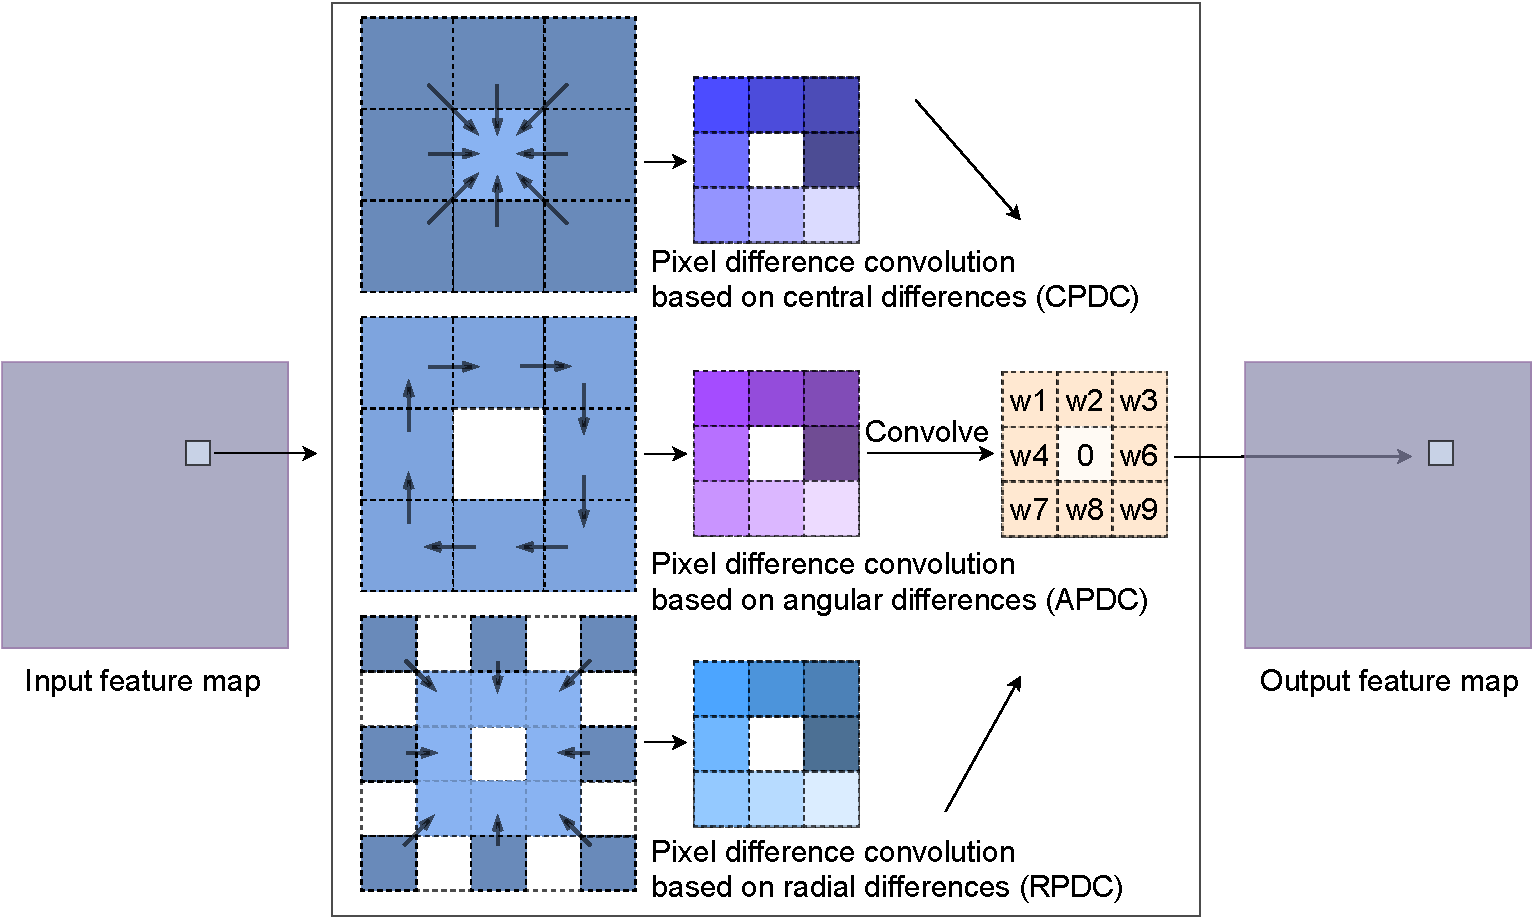
\includegraphics[width=1\linewidth]{images/pdc.pdf}
    % \caption{Three instances of pixel difference convolution derived from extended LBP descriptors~\cite{liu2011sorted, liu2012extended, su2019bird}. One can derive other instances by designing the picking strategy of the pixel pairs.}
    \caption{从扩展LBP描述符~\cite{liu2011sorted, liu2012extended, su2019bird}导出的三个像素差分卷积实例。可以通过设计像素对的拾取策略来推导出其他实例。}
    \label{fig:pdc}
\end{figure}

% The process of pixel difference convolution (PDC) is pretty similar to that of vanilla convolution, where the original pixels in the local feature map patch covered by the convolution kernels are replaced by pixel differences, when conducting the convolutional operation. The formulations of vanilla convolution and PDC can be written as:
像素差分卷积(PDC)的过程与普通卷积非常相似,在进行卷积运算时,卷积核覆盖的局部特征图补丁中的原始像素被像素差分替换。普通卷积和PDC的公式可以写成:
\begin{align}
    y &= f(\pmb{x}, \pmb{\theta}) = \sum_{i=1}^{k\times k}w_{i}\cdot x_{i}, \;\;\;\;\;\;\; \text{(vanilla convolution)} \\
    y &= f(\triangledown\pmb{x}, \pmb{\theta}) = \sum_{(x_i, x_i')\in \pmb{\mathcal{P}}}w_{i}\cdot (x_i - x_i'), \;\;\;\;\;\;\, \text{(PDC)} \label{eq: pdc}
\end{align}
% where, $x_i$ and $x_i'$ are the input pixels, $w_i$ is the weight in the $k \times k$ convolution kernel. $\pmb{\mathcal{P}} = \{(x_1, x_1'), (x_2, x_2'), ..., (x_m, x_m')\}$ is the set of pixel pairs picked from the current local patch, and $m\le k\times k$.
其中,$ x_i $和$ x_i' $是输入像素,$ w_i $是$ k \times k $卷积核中的权重。$ \pmb{\mathcal{P}} = \{(x_1, x_1'), (x_2, x_2'), ..., (x_m, x_m')\} $是从当前局部补丁选取的像素对集合,$ m \le k \times k $。

% To capture rich gradient information, the pixel pairs can be selected according to different strategies, which can be inspired from the numerous traditional feature descriptors. Here, we utilize the ideas from the work in~\cite{ojala2002lbp,liu2012extended,su2019bird}, where the local binary pattern (LBP) and its robust variants, extended LBP (ELBP), were used to encode pixel relations from varying directions (angular and radial). Specifically, ELBP are obtained by firstly calculating the pixel differences within a local patch (from $m$ pixel pairs), resulting in a pixel difference vector, and then binarizing the vector to create an $m$-length 0/1 code. Then, the bag-of-words technique~\cite{liu2019bow} is usually used to calculate the code distribution (or histogram), which is regarded as the image representation. In ELBP, the angular and radial directions were will demonstrated to help encode potential discriminative image cues and be complementary for increasing the feature representational capacity for various computer vision tasks, such as texture classification~\cite{liu2012extended,liu2011sorted} and face recognition~\cite{su2019bird}.
为了捕获丰富的梯度信息,可以根据不同的策略选择像素对,这可以从众多的传统特征描述符中得到启发。在这里,我们利用了~\cite{ojala2002lbp, liu2012extended, su2019bird}中的工作思想,其中局部二进制模式(LBP)及其稳健的变体扩展LBP(ELBP)用于从不同方向编码像素关系(角度和径向)。具体来说,ELBP是通过首先计算局部补丁内的像素差分(从$ m $个像素对)得到像素差分向量,然后将该向量二值化以创建长度为$ m $的0/1代码。然后,通常使用bag-of-words技术~\cite{liu2019bow}来计算代码分布(或直方图),作为图像表示。在ELBP中,角度和径向方向将被证明有助于编码潜在的判别性图像线索,并补充用于增加各种计算机视觉任务的特征表示能力,例如纹理分类~\cite{liu2012extended, liu2011sorted}和人脸识别~\cite{su2019bird}。

% By integrating ELBP with CNN convolution, we derive three types of PDC instances as shown in Fig.~\ref{fig:pdc}, in which we name them as central PDC (CPDC), angular PDC (APDC) and radial PDC (RPDC) respectively. The pixel pairs in the local patch is easy to understand. For example, for the APDC with kernel size $3\times 3$, we create 8 pairs in the angular direction in the $3\times 3$ local patch (thus $m=8$), then the pixel differences obtained from the pairs are convolved with the kernel by doing an element-wise multiplication with the kernel weights, followed by a summation, to generate the value in the output feature map.
通过将ELBP与CNN卷积相结合,我们得到了三种类型的PDC实例,如Fig. ~\ref{fig:pdc},其中我们分别将它们命名为中心PDC(CPDC)、角度PDC(APDC)和径向PDC(RPDC)。局部补丁中的像素对很容易理解。例如,对于卷积核大小为$ 3 \times 3 $的APDC,我们在$ 3\times 3 $局部补丁的角度方向上创建8个像素对(因此$ m = 8 $),然后把从像素对中获得的像素差分通过与卷积核权重进行逐元素乘法进行卷积,再求和,以生成输出特征图中的值。

% The derived PDC instances based on ELBP can be seen as an extension of ELBP that are more flexible and learnable. Although being powerful, the original ELBP codes are discrete with limited representative ability. While the useful encodings of pixel relations in PDC will be preserved in the trained convolution kernels, as during the training process of CNN, the convolution kernels will be encouraged to have higher inner product with those important encodings, in order to create higher activation responses\footnote{Usually, higher activation responses are considered to be more salient, as adopted in many network pruning methods~\cite{han2015deepcompression,su2020dynamic}}. By training from abundant of data, PDC is able to automatically learn rich representative encodings for the task.
基于ELBP的派生PDC实例可以看作是ELBP的扩展,更加灵活、更易于学习。虽然功能强大,但原始ELBP代码是离散的,代表能力有限。虽然PDC中像素关系的有用编码将保留在训练的卷积核中,但在CNN的训练过程中,将鼓励卷积核与那些重要的编码具有更高的内积,以创建更高的激活响应\footnote{通常,更高的激活响应被认为更显著,正如许多网络剪枝方法所采用的那样~\cite{han2015deepcompression, su2020dynamic}}。通过从大量数据中进行训练,PDC能够自动学习任务的丰富代表性编码。

\begin{figure}[h]
    \centering
    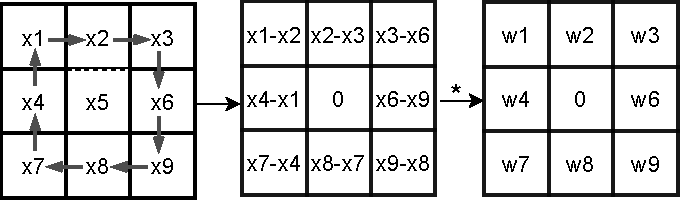
\includegraphics[width=0.8\linewidth]{images/APDC.pdf}
    % \caption{Selection of pixel pairs and convolution in APDC.}
    \caption{APDC中像素对的选择和卷积。}
    \label{fig:apdc}
\end{figure}

\vspace{0.3em}
% \noindent \textbf{Converting PDC to Vanilla Convolution.} \quad According to Eq.~\ref{eq: pdc}, one may notice that the computational cost and memory footprint by PDC are doubled compared with the vanilla counterpart. However, once the convolution kernels have been learnt, PDC layers can be converted to vanilla convolutional layers by instead saving the differences of the kernel weights in the model, according to the locations of the selected pixel pairs. In this way, the efficiency is maintained during inference. Taking APDC as an example (Fig.~\ref{fig:apdc}), conversion is done with the following equations:
\noindent \textbf{将PDC转换为普通卷积。} \quad 根据Eq. ~\ref{eq: pdc},人们可能会注意到PDC的计算成本和内存占用量与普通版本相比高出一倍。但是,一旦学习了卷积核,就可以根据所选像素对的位置,通过在模型中保存卷积核权重的差分,将PDC层转换为普通卷积层。这样,在推理过程中保持了效率。以APDC为例(Fig. ~\ref{fig:apdc}),转换是通过以下等式完成的:
{\small 
\begin{align}
    y &= w_{1}\cdot (x_1 - x_2) + w_2\cdot (x_2 - x_3)+w_3\cdot (x_3 - x_6) + ... \nonumber\\
    &=(w_1 - w_4)\cdot x_1 + (w_2 - w_1)\cdot x_2 + (w_3 - w_2)\cdot x_3 + ...\nonumber\\
    &=\hat{w}_1\cdot x_1 + \hat{w}_2\cdot x_2 + \hat{w}_3\cdot x_3 + ... =\sum \hat{w}_i\cdot x_i.
\end{align}
}

% It is worth mentioning that we can also use this tweak to speed up the training process, where the differences of kernel weights are firstly calculated, followed by the convolution with the untouched input feature maps. We have illustrated more details in the appendix.
值得一提的是,我们还可以使用此调整来加快训练过程,首先计算卷积核权重的差分,然后与未触及的输入特征图进行卷积。我们在附录中说明了更多细节。


% \section{PiDiNet Architecture}
\section{PiDiNet结构}


\begin{figure*}[t!]
    \centering
    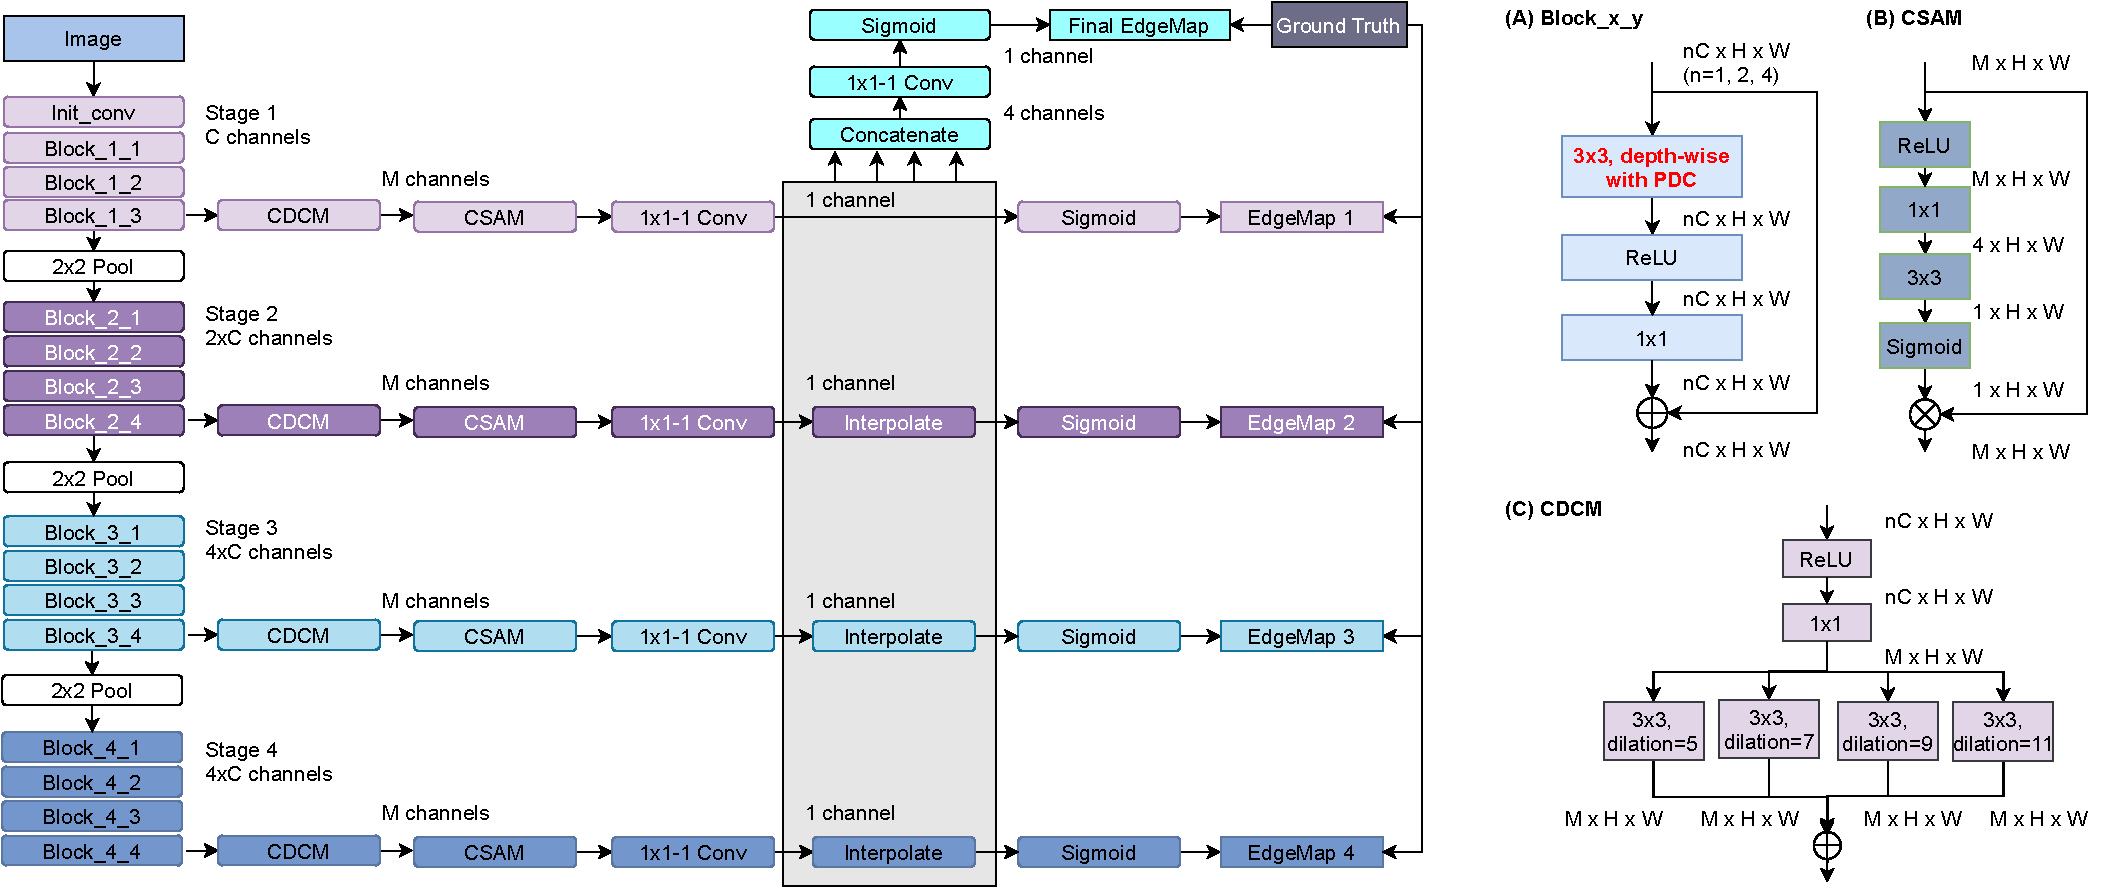
\includegraphics[width=0.98\linewidth]{images/arch.pdf}
    % \caption{PiDiNet architecture.}
    \caption{PiDiNet结构。}
    \label{fig:arch}
\end{figure*}


As tried by some prior works~\cite{wibisono2020fined,poma2020dense,wibisono2020traditional}, we believe it is both necessary and feasible to solve the inefficiency issues mentioned in Section~\ref{sec:intro} in one time by building an architecture with small model size and high running efficiency, and can be trained from scratch using limited datasets for effective edge detection. We construct our architecture with the following parts (Fig.~\ref{fig:arch}).

\vspace{0.3em}
\noindent \textbf{Efficient Backbone.} \quad The building principle for the backbone is to make the structure slim while own high running efficiency. Thus we do not consider the sophisticated multi-branch lightweight structures proposed for many other tasks~\cite{gao2020100k,mehta2019espnetv2,yu2018bisenet}, since they may not appeal to parallel implementation~\cite{ma2018shufflenetv2}, leading to unsatisfactory efficiency for the edge detection task. Inspired from \cite{he2016residual} and \cite{howard2017mobilenets}, we use the separable depth-wise convolutional structure with a shortcut for fast inference and easy training. The whole backbone has 4 stages and max pooling layers are among them for down sampling. Each stage has 4 residual blocks (except the first stage that has an initial convolutional layer and 3 residual blocks). The residual path in each block includes a depth-wise convolutional layer, a ReLU layer, and a point-wise convolutional layer sequentially. The number of channels in each stage is reasonably small to avoid big model size ($C$, $2\times C$, $4\times C$ and $4\times C$ channels for stage 1, 2, 3, and 4 respectively).

\vspace{0.3em}
\noindent \textbf{Efficient Side Structure.} \quad To learn rich hierarchical edge representation, we also use the side structure as in~\cite{xie2017holistically} to generate an edge map from each stage respectively, based on which a side loss is computed with the ground truth map to provide deep supervision~\cite{xie2017holistically}. To refine the feature maps, beginning from the end of each stage, we firstly build a compact dilation convolution based module (CDCM) to enrich multi-scale edge information, which takes the input with $n\times C$ channels, and produces $M$ ($M < C$) channels in the output to relieve the computation overhead, followed by a compact spatial attention module (CSAM) to eliminate the background noise. After that, a $1\times 1$ convolutional layer further reduces the feature volume to a single channel map, which is then interpolated to the original size followed by a Sigmoid function to create the edge map. The final edge map, which is used for testing, is created by fusing the 4 single channel feature maps with a concatenation, a convolutional layer and a Sigmoid function. 

The detailed structure information can be seen in Fig.~\ref{fig:arch}, noting that we do not use any normalization layers for simplicity since the resolutions of the training images are not uniform. The obtained architecture is our baseline. By replacing the vanilla convolution in the $3\times 3$ depth-wise convolutional layer in the residual blocks with PDC, we get the proposed PiDiNet.

\vspace{0.3em}
\noindent \textbf{Loss Function.} \quad We adopt the annotator-robust loss function proposed in~\cite{liu2019richer} for each generated edge map (including the final edge map). For the $i$th pixel in the $j$th edge map with value $p_i^j$, the loss is calculated as:
{\small \begin{equation}
    l_i^j = \begin{cases} 
    \alpha\cdot \log (1 - p_i^j) &\text{if } y_i  = 0 \\
    0 &\text{if } 0 < y_i < \eta \\
    \beta\cdot \log p_i^j &\text{otherwise},
    \end{cases}
\end{equation}}
where $y_i$ is the ground truth edge probability, $\eta$ is a pre-defined threshold, meaning that a pixel is discarded and not considered to be a sample when calculating the loss if it is marked as positive by fewer than $\eta$ of annotators to avoid confusing, $\beta$ is the percentage of negative pixel samples and $\alpha = \lambda\cdot (1-\beta)$. After all, the total loss is $L = \sum_{i,j}l_i^j$.


\section{Experiments}
\label{sec:experiments}

\subsection{Datasets and Implementation}
\noindent \textbf{Experimental Datasets.} \quad We evaluate the proposed PiDiNet on three widely used datasets, namely, BSDS500~\cite{arbelaez2010bsds}, NYUD~\cite{shi2000nyud}, and Multicue~\cite{mely2016multicue}. The experimental settings about data augmentation and configuration on the three datasets follow~\cite{xie2017holistically,liu2019richer,he2019bidirectional} and the details are given below. BSDS500 consists of 200, 100, and 200 images in the training set, validation set, and test set respectively. Each image has 4 to 9 annotators. Training images in the dataset are augmented with flipping (2$\times$), scaling (3$\times$), and rotation (16$\times$), leading to a training set that is 96$\times$ larger than the unaugmented version. Like prior works~\cite{xie2017holistically,liu2019richer,he2019bidirectional}, the PASCAL VOC Context dataset~\cite{mottaghi2014voc}, which has 10K labeled images (and augmented to 20K with flipping), is also optionally considered in training. NYUD has 1449 pairs of aligned RGB and depth images which are densely labeled. There are 381, 414 and 654 images for training, validation, and test respectively. We combine the training and validation set and augment them with flipping (2$\times$), scaling (3$\times$), and rotation (4$\times$) to produce the training data. Multicue is composed of 100 challenging natural scenes and each scene contains a left- and right-view color sequences captured by a binocular stereo camera. The last frame of left-view sequences for each scene, which is labeled with edges and boundaries, is used in our experiments. We randomly split them to 80 and 20 images for training and evaluation respectively. The process is independently repeated twice more. The metrics are then recorded from the three runs. We also augment each training image with flipping (2$\times$), scaling (3$\times$), and rotation ($16\times$), then randomly crop them with size 500$\times$500. 


\vspace{0.3em}
\noindent \textbf{Performance Metrics.} \quad During evaluation, \emph{F-measure} at both Optimal Dataset Scale (ODS) and Optimal Image Scale (OIS) are recorded for all datasets. Since efficiency is one of the main focuses in this paper, all the models are compared based on the evaluations from single scale images if not specified.


\vspace{0.3em}
\noindent \textbf{Implementation Details.} \quad Our implementation is based on the Pytorch library~\cite{paszke2019pytorch}. In detail, PiDiNet (and the baseline) is randomly initialized and trained for 14 epochs with Adam optimizer~\cite{kingma2014adam} with an initial learning rate 0.005, which is decayed in a multi-step way (at epoch 8 and 12 with decaying rate 0.1). If VOC dataset is used in training for evaluating BSDS500, we train 20 epochs and decay the learning rate at epoch 10 and 16. $\lambda$ is set to 1.1 for both BSDS500 and Multicue, and 1.3 for NYUD. The threshold $\eta$ is set to 0.3 for both BSDS500 and Multicue. No $\eta$ is needed for NYUD since the images are singly annotated. 

\begin{table}[t!]
\caption{Possible configurations of PiDiNet. `C', `A', `R' and `V' indicate CPDC, APDC, RPDC and vanilla convolution respectively. `$\times$n' means repeating the pattern for $n$ times sequentially. For example, the baseline architectrue can be presented as ``[V]$\times$16'', and `C-[V]$\times$15' means using CPDC in the first block and vanilla convolutions in the later blocks. All the models are trained using BSDS500 training set and the VOC dataset, then evaluated on BSDS500 validation set.}
\begin{center}
\setlength{\tabcolsep}{0.05\linewidth}
\resizebox*{\linewidth}{!}{
\begin{tabular}{l||l|l|l}
\toprule[1pt]
Architecture & C-[V]$\times$15 & A-[V]$\times$15 & R-[V]$\times$15 \\
\hline
ODS / OIS & 0.775 / 0.794 & 0.774 / 0.794 & 0.774 / 0.792 \\
\hline
Architecture & [CVVV]$\times$4 & [AVVV]$\times$4 & [RVVV]$\times$4 \\
\hline
ODS / OIS & 0.773 / 0.792 & 0.771 / 0.790 & 0.772 / 0.791 \\
\hline
Architecture & [CCCV]$\times$4 & [AAAV]$\times$4 & [RRRV]$\times$4 \\
\hline
ODS / OIS & 0.772 / 0.791 & 0.775 / 0.793 & 0.771 / 0.787 \\
\hline
Architecture & [C]$\times$16 & [A]$\times$16 & [R]$\times$16 \\
\hline
ODS / OIS & 0.767 / 0.786 & 0.768 / 0.786 & 0.758 / 0.777 \\
\hline
Architecture & Baseline & \multicolumn{2}{l}{\textbf{[CARV]$\times$4 (PiDiNet)}} \\
\hline
ODS / OIS & 0.772 / 0.792 & \multicolumn{2}{l}{\textbf{0.776 / 0.795}} \\
\bottomrule[1pt]
\end{tabular}
}
\end{center}
\label{table:configuration}
\end{table}


\begin{table}[t!]
\caption{More comparisons between PiDiNet and the baseline architecture in multiple network scales by changing the nubmer of channels $C$ (see Fig.~\ref{fig:arch}). The models are trained using the BSDS500 training set, and evaluated on BSDS500 validation set.}
\begin{center}
\setlength{\tabcolsep}{0.05\linewidth}
\resizebox*{\linewidth}{!}{
\begin{tabular}{l|c|c}
\toprule[1pt]
Scale & Baseline (ODS / OIS) & PiDiNet (ODS / OIS) \\
\hline
Tiny (C=20) & 0.735 / 0.752 & \textbf{0.747 / 0.764} \\
\hline
Small (C=30) & 0.738 / 0.759 & \textbf{0.752 / 0.769} \\
\hline
Normal (C=60) & 0.736 / 0.751 & \textbf{0.757 / 0.776} \\
\bottomrule[1pt]
\end{tabular}
}
\end{center}
\label{table:morecomparison}
\end{table}


\begin{table}[t!]
\caption{Ablation on CDCM, CSAM and shortcuts. The models are trained with BSDS500 training set and VOC dataset, and evaluated on BSDS500 validation set.}
\begin{center}
\setlength{\tabcolsep}{0.08\linewidth}
\resizebox*{\linewidth}{!}{
\begin{tabular}{ccc|c}
\toprule[1pt]
CSAM & CDCM & Shortcuts & ODS / OIS \\
\hline
\xmark & \xmark & \cmark & 0.770 / 0.790 \\
\hline
\xmark & \cmark & \cmark & 0.775 / 0.793 \\
\hline
\cmark & \cmark & \cmark & \textbf{0.776 / 0.795} \\
\hline
\cmark & \cmark & \xmark & 0.734 / 0.755 \\
\bottomrule[1pt]
\end{tabular}
}
\end{center}
\label{table:moreablation}
\end{table}


\subsection{Ablation Study}
To demonstrate the effectiveness of PDC and to find the possibly optimal architecture configuration, we conduct our ablation study on the BSDS500 dataset, where we use the data augmented from the 200 images in the training set (optionally mixed with the VOC dataset) for training and record the metrics on the validation set. 

\vspace{0.3em}
\noindent \textbf{Architecture Configuration.} \quad We can replace the vanilla convolution with PDC in any block (we also regard the initial convolutional layer as a block in the context) in the backbone. Since there are 16 blocks, and a brute force search for the architecture configurations is not feasible, hence we only sample some of them as shown in Table~\ref{table:configuration} by gradually increasing the number of PDCs. We found replacing the vanilla convolution with PDC only in a single block can even have obvious improvement. More replacements with the same type of PDC may no longer give extra performance gain and instead degenerate the model. We conjecture that the PDC in the first block already obtains much gradient information from the raw image, and an abuse of PDC may even cause the model fail to preserve useful information. The extreme case is that when all the blocks are configured with PDC, the performance becomes worse than that of the baseline. The best configuration is `[CARV]$\times$4', which means combing the 4 types of convolutions sequentially in each stage, as different types of PDC capture the gradient information in different encoding directions. We will use this configuration in the following experiments. 

To further demonstrate the superiority of PiDiNet over the baseline, which only uses the vanilla convolution, we give more comparisons as shown in Table~\ref{table:morecomparison}. It constantly proves that PDC configured architectures outperform the corresponding vanilla convolution configured architectures.

\vspace{0.3em}
\noindent \textbf{CSAM, CDCM and Shortcuts.} \quad The effectiveness of CSAM, CDCM and residual structures are demonstrated in Table~\ref{table:moreablation}. The addition of shortcuts is simple yet important, as they can help preserve the gradient information captured by the previous layers. On the other hand, the attention mechanism in CSAM and dilation convolution in CDCM can give extra performance gains, while may also bring some computational cost. Therefore, they can be used to tradeoff between accuracy and efficiency. In the following experiments, we note PiDiNet without CSAM and CDCM as PiDiNet-L (meaning a more lightweight version).

\begin{figure}[t!]
    \centering
    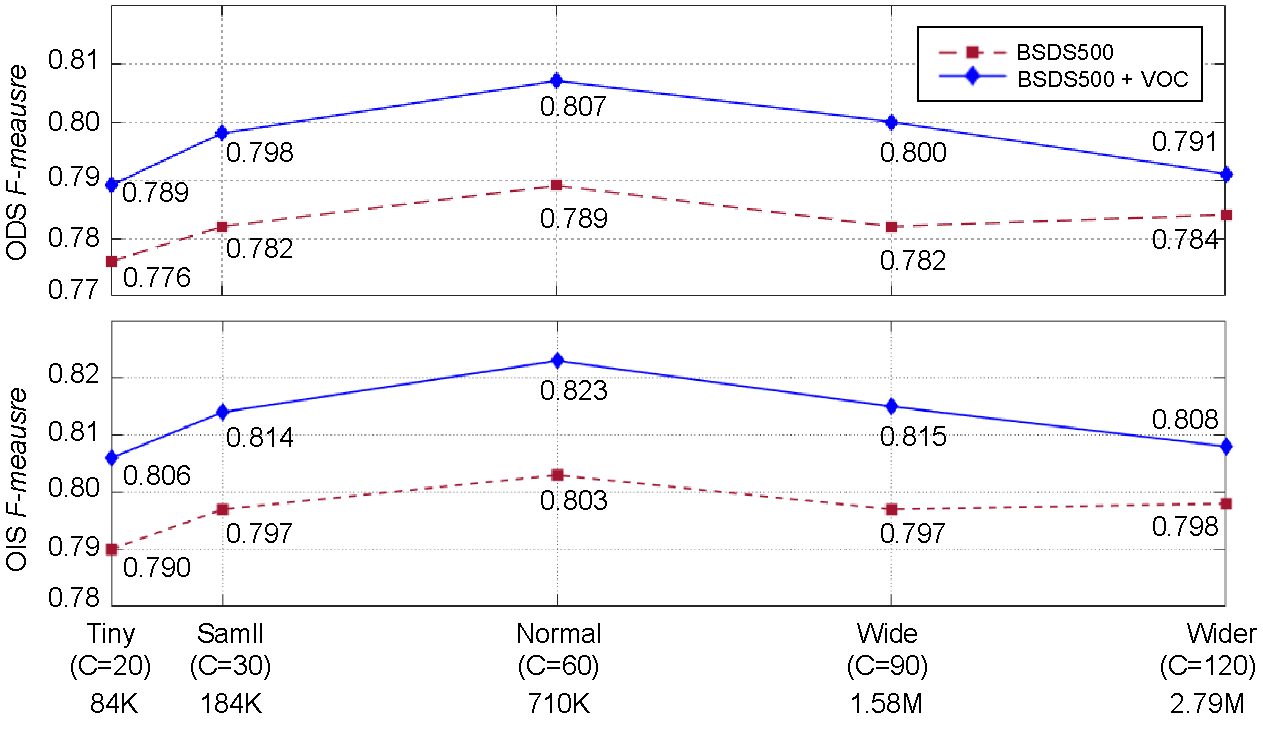
\includegraphics[width=1\linewidth]{images/ex_1.pdf}
    \caption{Exploration on the scalability of PiDiNet. The structure sizes are changed by slimming or widening the basic PiDiNet. Bottom row shows the number of parameters for each model. The models are trained with or without VOC dataset.}
    \label{fig:scalability}
\end{figure}

\begin{figure*}[t!]
    \centering
    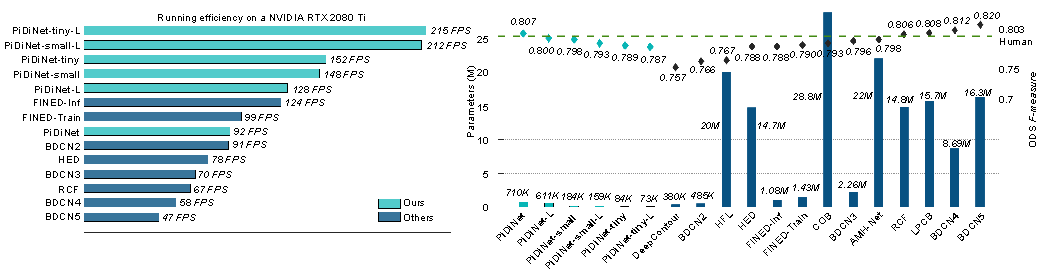
\includegraphics[width=1\linewidth]{images/fps_param.pdf}
    \caption{Comparison with other methods in terms of network complexity, running efficiency and detection performance (on BSDS500 dataset). The running speeds of FINED~\cite{wibisono2020fined} are cited from the original paper, and the rest are evaluated by our implementations}
    \label{fig:efficient}
\end{figure*}

\begin{table}[t!]
\caption{Comparison with other methods on BSDS500 dataset. $^\ddagger$ indicates the speeds with our implementations based on a NVIDIA RTX 2080 Ti GPU. $^\dagger$ indicates the cited GPU speeds.}
\begin{center}
\setlength{\tabcolsep}{0.04\linewidth}
\resizebox*{0.82\linewidth}{!}{
\begin{tabular}{l|c|c|c}
\toprule[1pt]
Method & ODS & OIS & FPS \\
\hline
Human & .803 & .803 & \\
\hline
Canny~\cite{canny1986computational} & .611 & .676 & 28 \\
Pb~\cite{martin2004pb} & .672 & .695 & - \\
SCG~\cite{xiaofeng2012scg} & .739 & .758 & - \\
SE~\cite{dollar2014se} & .743 & .763 & 12.5 \\
OEF~\cite{hallman2015oef} & .746 & .770 & 2/3 \\
\hline
DeepEdge~\cite{bertasius2015deepedge} & .753 & .772 & 1/1000$^\dagger$ \\
DeepContour~\cite{shen2015deepcontour} & .757 & .776 & 1/30$^\dagger$ \\
HFL~\cite{bertasius2015hfl} & .767 & .788 & 5/6$^\dagger$ \\
CEDN~\cite{yang2016cedn} & .788 & .804 & 10$^\dagger$ \\
HED~\cite{xie2017holistically} & .788 & .808 & 78$^\ddagger$ \\
DeepBoundary~\cite{kokkinos2015deepboundary} & .789 & .811 & -\\
COB~\cite{maninis2016cob} & .793 & .820 & - \\
CED~\cite{wang2017ced} & .794 & .811 & - \\
AMH-Net~\cite{xu2018amhnet} & .798 & .829 & - \\
RCF~\cite{liu2019richer} & .806 & .823 & 67$^\ddagger$ \\
LPCB~\cite{deng2018lpcb} & .808 & .824 & 30$^\dagger$ \\
BDCN~\cite{he2019bidirectional} & .820 & .838 & 47$^\ddagger$ \\
\hline
FINED-Inf~\cite{wibisono2020fined} & .788 & .804 & 124$^\dagger$ \\
FINED-Train~\cite{wibisono2020fined} & .790 & .808 & 99$^\dagger$ \\
\hline
Baseline & .798 & .816 & 96$^{\ddagger}$ \\
PiDiNet & .807 & .823 & 92$^{\ddagger,\ast}$ \\
PiDiNet-L & .800 & .815 & 128$^\ddagger$ \\
PiDiNet-Small & .798 & .814 & 148$^\ddagger$ \\
PiDiNet-Small-L & .793 & .809 & 212$^\ddagger$ \\
PiDiNet-Tiny & .789 & .806 & 152$^\ddagger$ \\
PiDiNet-Tiny-L & .787 & .804 & 215$^\ddagger$ \\
\bottomrule[1pt]
\multicolumn{4}{l}{\footnotesize{$^\ast$ ``PiDiNet'' is slightly slower than ``Baseline'' because RPDC is}}\\
\multicolumn{4}{l}{\footnotesize{a 5x5 convolution after conversion.}}
\end{tabular}
}
\end{center}
\label{table:bsds}
\vspace{-0.2in}
\end{table}


\subsection{Network Scalability}
\label{sec:scalability}
PiDiNet is highly compact with only 710K parameters and support training from scratch with limited training data. Here, we explore the scalability of PiDiNet with different model complexities as shown in Fig.~\ref{fig:scalability}. In order to compare with other approaches, the models are trained in two schemes, both use the BSDS500 training and validation set, while with or without mixing the VOC dataset during training. Metrics are recorded on BSDS500 test set. As expected, compared with the basic PiDiNet, smaller models suffer from lower network capacity and thus with degenerated performances in terms of both ODS and OIS scores. At the same time, training with more data constantly leads to higher accuracy. It is noted that the normal scale PiDiNet, can achieve the ODS and OIS scores at the same level as that recorded in the HED approach~\cite{xie2017holistically}, even when trained from scratch only using the BSDS500 dataset (\emph{i.e.}, 0.789 vs. 0.788 in ODS and 0.803 vs. 0.808 in OIS for PiDiNet vs. HED). However, with limited training data, widening the PiDiNet architecture may cause the overfitting problem, as shown in the declines in the second half of the curves. In the following experiments, we only use the tiny, small, and normal versions of PiDiNet, dubbed as PiDiNet-Tiny, PiDiNet-Small and PiDiNet respectively.




\begin{figure}[t!]
    \centering
    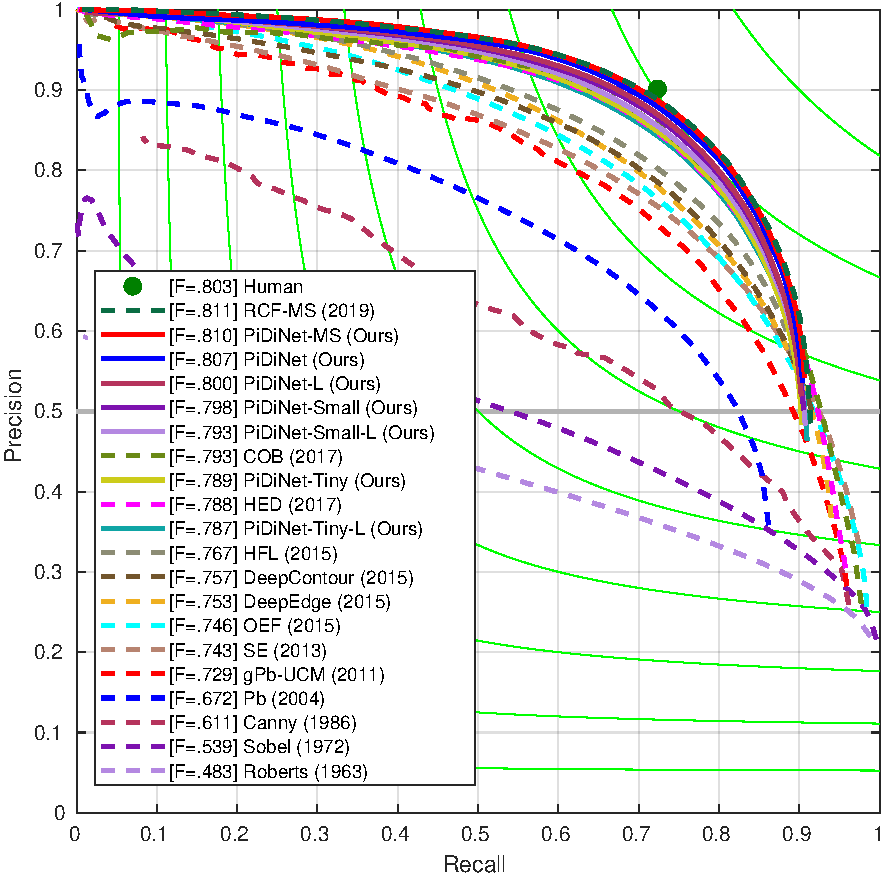
\includegraphics[width=1\linewidth]{images/bsds_pr.pdf}
    \caption{Precision-Recall curves of our models and some competitors on BSDS500 dataset.}
    \label{fig:bsds_pr}
\end{figure}



\subsection{Comparison with State-of-the-arts}

\vspace{0.3em}
\noindent \textbf{On BSDS500 dataset.} \quad We compare our methods with prior edge detection approaches including both traditional ones and recently proposed CNN based ones, as summarized in Table~\ref{table:bsds} and Fig.~\ref{fig:bsds_pr}. Firstly, we notice that our baseline model can even achieve comparable results, \emph{i.e.}, with ODS of 0.798 and OIS of 0.816, already beating most CNN based models like CED~\cite{wang2017ced}, DeepBoundary~\cite{kokkinos2015deepboundary} and HED~\cite{xie2017holistically}. With PDC, PiDiNet can further boost the performance with ODS of 0.807, being the same level as the recently proposed RCF~\cite{liu2019richer} while still achieving nearly 100 FPS. The fastest version PiDiNet-Tiny-L, can also achieve comparable prediction performance with more than 200 FPS, further demonstrating the effectiveness of our methods. Noting all of our modes are trained from scratch using the same amount of training data as in RCF, LPCB, BDCN, \emph{etc}. (\emph{i.e.}, the training and validation set, mixed with the VOC dataset), without the ImageNet pretraining. We also show some qualitative results in Figure~\ref{fig:bsds_visualization}. A more detailed comparison in terms of network complexity, running efficiency and accuracy can be seen in Fig.~\ref{fig:efficient}. 

\vspace{0.3em}
\noindent \textbf{On NYUD dataset.} \quad The comparison results on the NYUD dataset are illustrated on Table~\ref{table:nyud}. Following the prior works, we get the `RGB-HHA' results by averaging the output edge maps from RGB image and HHA image to get the final edge map. The quantitative comparison shows that PiDiNets can still achieve highly comparable results among the state-of-the-art methods while being efficient. Please refer to the appendix for the Precision-Recall curves.

\vspace{0.3em}
\noindent \textbf{On Multicue dataset.} \quad We also record the evaluation results on Multicue dataset and the comparison results with other methods are shown on Table~\ref{table:multicue}. Still, PiDiNets achieve promising results with high efficiencies.


\begin{table}[t!]
\caption{Comparison with other methods on NYUD dataset. $^\ddagger$ indicates the speeds with our implementations based on a NVIDIA RTX 2080 Ti GPU.}
\vspace{-0.1in}
\begin{center}
\setlength{\tabcolsep}{0.025\linewidth}
\resizebox*{\linewidth}{!}{
\begin{tabular}{l|c|c|c|c|c|c|c}
\toprule[1pt]
Methods & ODS & OIS & ODS & OIS & ODS & OIS & FPS \\
\hline 
gPb-UCM~\cite{arbelaez2010bsds} & .632 & .661 & & & & & 1/360 \\
gPb+NG~\cite{gupta2013gpbng} & .687 & .716 & & & & & 1/375 \\
SE~\cite{dollar2014se} & .695 & .708 & & & & & 5 \\
SE+NG+~\cite{gupta2014seng} & .710 & .723 & & & & & 1/15 \\
\hline
\hline
& \multicolumn{2}{c|}{RGB} & \multicolumn{2}{c|}{HHA} & \multicolumn{2}{c|}{RGB-HHA} & \\
\hline
HED~\cite{xie2017holistically} & .720 & .734 & .682 & .695 & .746 & .761 & 62$^\ddagger$ \\
LPCB~\cite{deng2018lpcb} & .739 & .754 & .707 & .719 & .762 & .778 & - \\
RCF~\cite{liu2019richer} & .743 & .757 & .703 & .717 & .765 & .780 & 52$^\ddagger$ \\
AMH-Net~\cite{xu2018amhnet} & .744 & .758 & .716 & .729 & .771 & .786 & - \\
BDCN~\cite{he2019bidirectional} & .748 & .763 & .707 & .719 & .765 & .781 & 33$^\ddagger$ \\
\hline
PiDiNet & .733 & .747 & .715 & .728 & . 756 & .773 & 62$^\ddagger$ \\
PiDiNet-L & .728 & .741 & .709 & .722 & .754 & .770 & 88$^\ddagger$ \\
PiDiNet-Small & .726 & .741 & .705 & .719 & .750 & .767 & 115$^\ddagger$ \\
PiDiNet-Small-L & .721 & .736 & .701 & .713 & .746 & .763 & 165$^\ddagger$ \\
PiDiNet-Tiny & .721 & .736 & .700 & .714 & .745 & .763 & 140$^\ddagger$ \\
PiDiNet-Tiny-L & .714 & .729 & .693 & .706 & .741 & .759 & 206$^\ddagger$ \\
\bottomrule[1pt]
\end{tabular}
}
\end{center}
\label{table:nyud}
\vspace{-0.1in}
\end{table}


\begin{table}[t!]
\caption{Comparison with other methods on Multicue dataset. $^\ddagger$ indicates the speeds with our implementations based on a NVIDIA RTX 2080 Ti GPU.}
\vspace{0.05in}
\begin{center}
\setlength{\tabcolsep}{0.015\linewidth}
\resizebox*{\linewidth}{!}{
\begin{tabular}{l|c|c|c|c|c}
\toprule[1pt]
Method & \multicolumn{2}{c|}{Boundary} & \multicolumn{2}{c|}{Edge} & FPS \\
\hhline{~----~}
 & ODS & OIS & ODS & OIS & \\
\hline 
Human~\cite{mely2016multicue} & .760 (.017) & & .750 (.024) &  & \\
\hline
Multicue~\cite{mely2016multicue} & .720 (.014) & & .830 (.002) & & - \\
HED~\cite{xie2017holistically} & .814 (.011) & .822 (.008) & .851 (.014) & .864 (.011) & 18$^\ddagger$ \\
RCF~\cite{liu2019richer} & .817 (.004) & .825 (.005) & .857 (.004) & .862 (.004) & 15$^\ddagger$ \\
BDCN~\cite{he2019bidirectional} & .836 (.001) & .846 (.003) & .891 (.001) & .898 (.002) & 9$^\ddagger$ \\
\hline
PiDiNet & .818 (.003) & .830 (.005) & .855 (.007) & .860 (.005) & 17$^\ddagger$ \\
PiDiNet-L & .810 (.005) & .822 (.002) & .854 (.007) & .860 (.004) & 23$^\ddagger$ \\
PiDiNet-Small & .812 (.004) & .825 (.004) & .858 (.007) & .863 (.004) & 31$^\ddagger$ \\
PiDiNet-Small-L & .805 (.007) & .818 (.002) & .854 (.007) & .860 (.004) & 44$^\ddagger$ \\
PiDiNet-Tiny & .807 (.007) & .819 (.004) & .856 (.006) & .862 (.003) & 43$^\ddagger$ \\
PiDiNet-Tiny-L & .798 (.007) & .811 (.005) & .854 (.008) & .861 (.004) & 56$^\ddagger$ \\
\bottomrule[1pt]
\end{tabular}
}
\end{center}
\label{table:multicue}
\end{table}


\begin{figure}[t!]
    \centering
    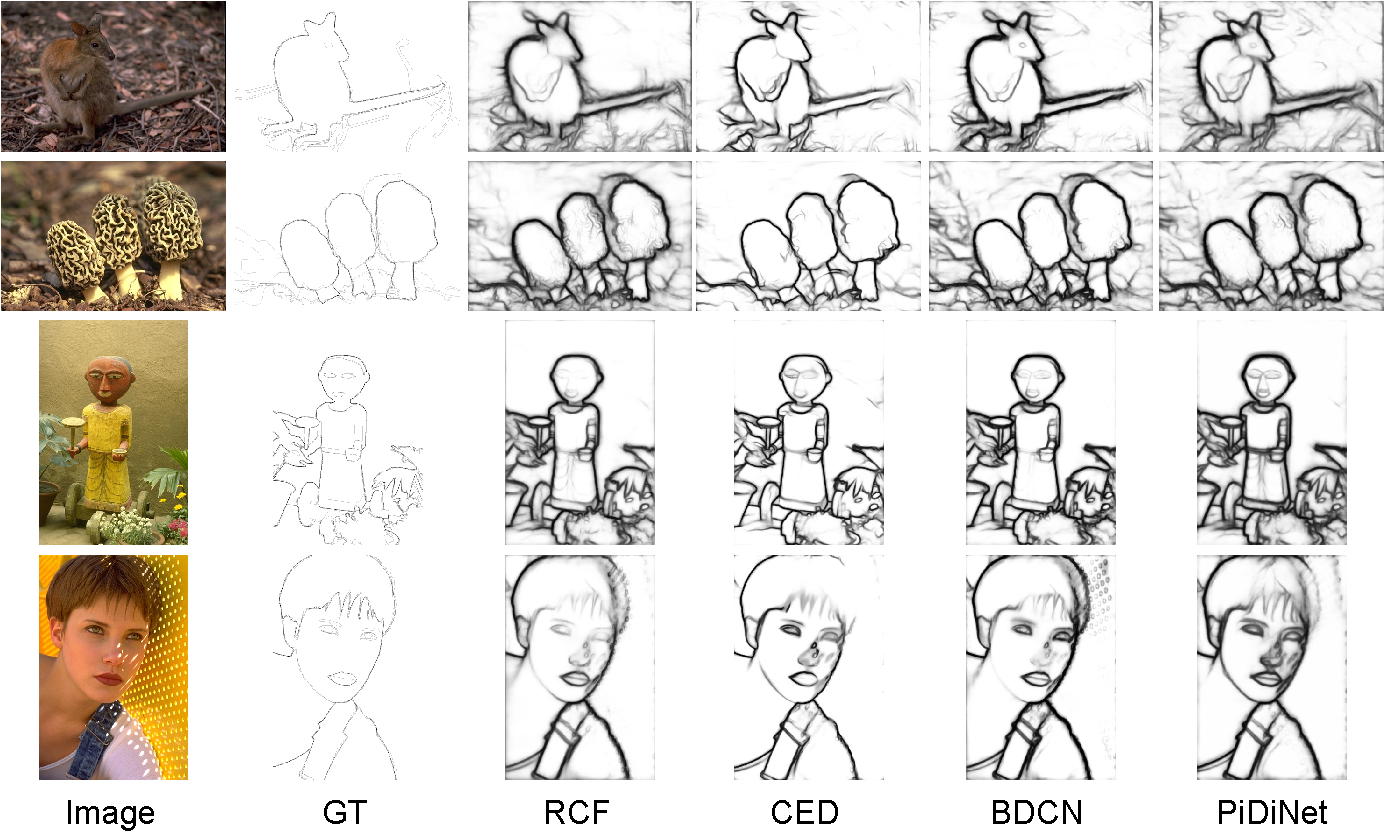
\includegraphics[width=1\linewidth]{images/vis3.pdf}
    \caption{A qualitative comparison of network outputs with some other methods, including RCF~\cite{liu2019richer}, CED~\cite{wang2017ced} and BDCN~\cite{he2019bidirectional}.}
    \label{fig:bsds_visualization}
\end{figure}


\section{Conclusion}
In conclusion, the contribution in this paper is three-fold: Firstly, we derive the pixel difference convolution which integrates the wisdom from the traditional edge detectors and the advantages of the deep CNNs, leading to robust and accurate edge detection. Secondly, we propose a highly efficient architecture named PiDiNet based on pixel difference convolution, which are memory friendly and with high inference speed. Furthermore, PiDiNet can be trained from scratch only using limited data samples, while achieving human-level performances, breaking the convention that high performance CNN based edge detectors usually need a backbone pretrained on large scale dataset. Thirdly, we conduct extensive experiments on BSDS500, NYUD, and Multicue datasets for edge detection. We believe that PiDiNet has created new state-of-the-art performances considering both accuracy and efficiency.

\vspace{0.5em}
\noindent \textbf{Future Work.} \quad As discussed in Section~\ref{sec:intro}, edge detection is a low level task for many mid- or high-level vision tasks like semantic segmentation and object detection. Also, some low level tasks like salient object detection may also benefit from the image boundary information. We hope pixel difference convolution and the proposed PiDiNet can go further and be useful in these related tasks. 

\vspace{0.5em}
\noindent \textbf{Acknowledgement.} \quad This work was partially supported by the Academy of Finland under grant 331883 and the National Natural Science Foundation of China under Grant 61872379, 62022091, and 71701205. The authors also wish to acknowledge CSC IT Center for Science, Finland, for computational resources.

{\small
\bibliographystyle{ieee_fullname}
\bibliography{main}
}

\clearpage


\section{Appendix}

\subsection{Converting Pixel Difference Convolution (PDC) to Vanilla Convolution}

The main goal of the conversion is to make PDC as fast and memory efficient as as the vanilla convolution. 
As introduced in the main paper, the formulations of vanilla convolution and PDC can be written as:

\begin{align}
    y &= f(\pmb{x}, \pmb{\theta}) = \sum_{i=1}^{k\times k}w_{i}\cdot x_{i}, \;\;\;\;\;\;\; \text{(vanilla convolution)}\label{eq:vanilla} \\
    y &= f(\triangledown\pmb{x}, \pmb{\theta}) = \sum_{(x_i, x_i')\in \pmb{\mathcal{P}}}w_{i}\cdot (x_i - x_i'), \;\;\;\;\;\;\, \text{(PDC)} \label{eq: pdc}
\end{align}
where, $x_i$ and $x_i'$ are the pixels in the current input local patch, $w_i$ is the weight in the $k \times k$ convolution kernel. $\pmb{\mathcal{P}} = \{(x_1, x_1'), (x_2, x_2'), ..., (x_m, x_m')\}$ is the set of pixel pairs picked from the local patch, and $m\le k\times k$. 

The conversion from PDC to vanilla convolution can be done in both the training and inference phases.

\vspace{0.3em}
\noindent  \textbf{Conversion in the Training Phase.} \quad Eq.~\ref{eq: pdc} can be transformed to fit the form of Eq.~\ref{eq:vanilla}, according to the selection strategies of the pixel pairs. Correspondingly, PDC can be converted to vanilla convolution by firstly transforming the kernel weights to a new set of kernel weights, followed by a vanilla convolutional operation. We will discuss Central PDC (CPDC), Angular PDC (APDC) and Radial PDC (RPDC) respectively.
The selection strategies of pixel pairs in the three PDC instances are shown in Fig.~\ref{fig:cpdc}, Fig.~\ref{fig:apdc} and Fig.~\ref{fig:rpdc}. The transformations of the equations are as follows.

\vspace{0.3em}
\noindent For CPDC (Fig.~\ref{fig:cpdc}):

\begin{figure}[t!]
    \centering
    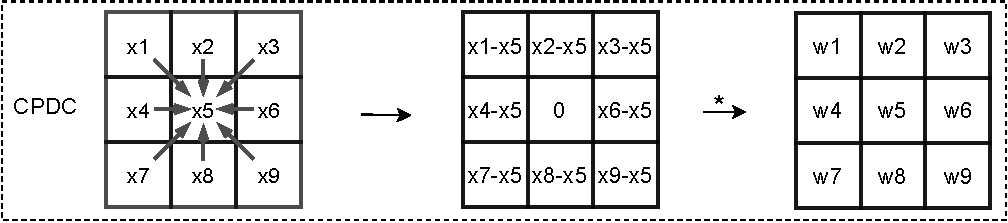
\includegraphics[width=0.95\linewidth]{images/supplement_cpdc.pdf}
    \caption{Selection of pixel pairs and convolution in CPDC.}
    \label{fig:cpdc}
\end{figure}


{\small 
\begin{align}
    y =& w_{1}\cdot (x_1 - x_5) + w_2\cdot (x_2 - x_5)+w_3\cdot (x_3 - x_5)\nonumber\\
    & + w_4\cdot (x_4-x_5) + w_6\cdot (x_6 - x_5) + w_7\cdot (x_7 - x_5)\nonumber \\
    & + w_8\cdot (x_8 - x_5) + w_9\cdot (x_9 - x_5)\nonumber \\
    =&w_1\cdot x_1 + w_2\cdot x_2 + w_3\cdot x_3 +\nonumber \\
    & + w_4\cdot x_4 + w_6\cdot x_6 + w_7\cdot x_7 +\nonumber \\
    & + w_8\cdot x_8 + w_9\cdot x_9\nonumber \\
    & + (-\sum_{i=\{1,2,3,4,6,7,8,9\}}w_i)\cdot x5\nonumber \\
    =&\hat{w}_1\cdot x_1 + \hat{w}_2\cdot x_2 + \hat{w}_3\cdot x_3 + ... =\sum \hat{w}_i\cdot x_i
\end{align}
}

\begin{figure}[t!]
    \centering
    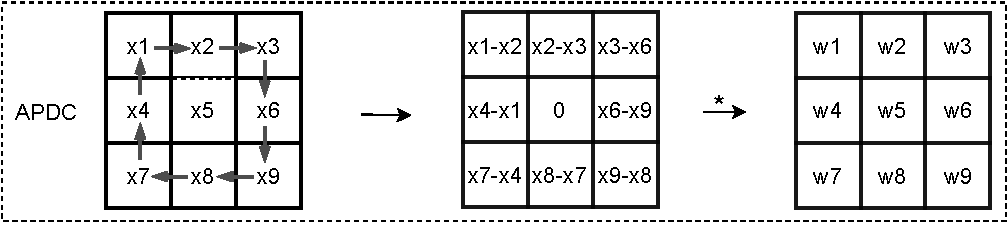
\includegraphics[width=0.95\linewidth]{images/supplement_apdc.pdf}
    \caption{Selection of pixel pairs and convolution in APDC.}
    \label{fig:apdc}
\end{figure}

\vspace{0.3em}
\noindent For APDC (Fig.~\ref{fig:apdc}):

{\small
\begin{align}
    y =& w_{1}\cdot (x_1 - x_2) + w_2\cdot (x_2 - x_3)+w_3\cdot (x_3 - x_6)\nonumber\\
    & + w_4\cdot (x_4-x_1) + w_6\cdot (x_6 - x_9) + w_7\cdot (x_7 - x_4)\nonumber \\
    & + w_8\cdot (x_8 - x_7) + w_9\cdot (x_9 - x_8)\nonumber \\
    =& (w_1 - w_4)\cdot x_1 + (w_2 - w_1)\cdot x_2 + (w_3-w_2)\cdot x_3 \nonumber \\
    & + (w_4 - w_7)\cdot x_4 + (w_6 - w_3)\cdot x_6 + (w_7 - w_8)\cdot x_7 \nonumber \\
    & + (w_8 - w_9)\cdot x_8 + (w_9 - x_6)\cdot x_9\nonumber \\
    & + 0\cdot x_5\nonumber \\
    =& \hat{w}_1\cdot x_1 + \hat{w}_2\cdot x_2 + \hat{w}_3\cdot x_3 + ... =\sum \hat{w}_i\cdot x_i
\end{align}
}

\begin{figure}[t!]
    \centering
    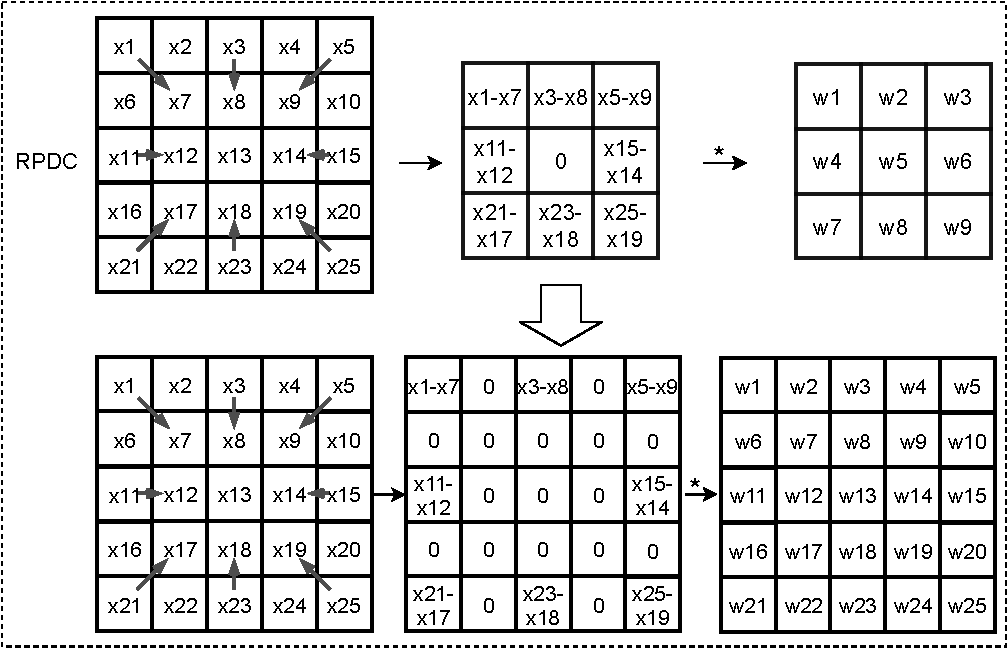
\includegraphics[width=0.95\linewidth]{images/supplement_rpdc.pdf}
    \caption{Selection of pixel pairs and convolution in RPDC.}
    \label{fig:rpdc}
\end{figure}

\vspace{0.3em}
\noindent For RPDC (Fig.~\ref{fig:rpdc}):

{\small
\begin{align}
    y =& w_{1}\cdot (x_1 - x_7) + w_3\cdot (x_3 - x_8)+w_5\cdot (x_5 - x_9)\nonumber\\
    & + w_{11}\cdot (x_{11}-x_{12}) + w_{15}\cdot (x_{15} - x_{14})\nonumber \\
    &  + w_{21}\cdot (x_{21} - x_{17}) + w_{23}\cdot (x_{23} - x_{18})\nonumber \\
    &  + w_{25}\cdot (x_{25} - x_{19})\nonumber\\
    =&w_1\cdot x_1 + w_3\cdot x_3 + w_5\cdot x_5\nonumber \\
    & + (-w_1)\cdot x_7 + (-w_3)\cdot x_8 + (-w_5)\cdot x_9 +\nonumber \\
    & + w_{11}\cdot x_{11} + (-w_{11})\cdot x_{12} + (-w_{15})\cdot x_{14}\nonumber\\
    & + w_{15}\cdot x_{15} + (-w_{21})\cdot x_{17} + (-w_{23})\cdot x_{18}\nonumber\\
    & + (-w_{25})\cdot x_{19} + w_{21}\cdot x_{21} + w_{23}\cdot x_{23}\nonumber\\
    & + w_{25}\cdot x_{25} + \sum_{i=\{2,4,6,10,13,16,20,22,24\}}0\cdot x_i\nonumber\\
    =&\hat{w}_1\cdot x_1 + \hat{w}_2\cdot x_2 + \hat{w}_3\cdot x_3 + ... =\sum \hat{w}_i\cdot x_i
\end{align}
}

The RPDC is converted to a vanilla convolution with kernel size $5\times 5$.

\vspace{0.3em}
\noindent  \textbf{Conversion in the Inference Phase.} \quad After training, instead of saving the original weights $w_i$, we directly save the new set of weights $\hat{w}_i$. Therefore, during inference, all the convolutional operations are vanilla convolutions.

\begin{figure}[t!]
    \centering
    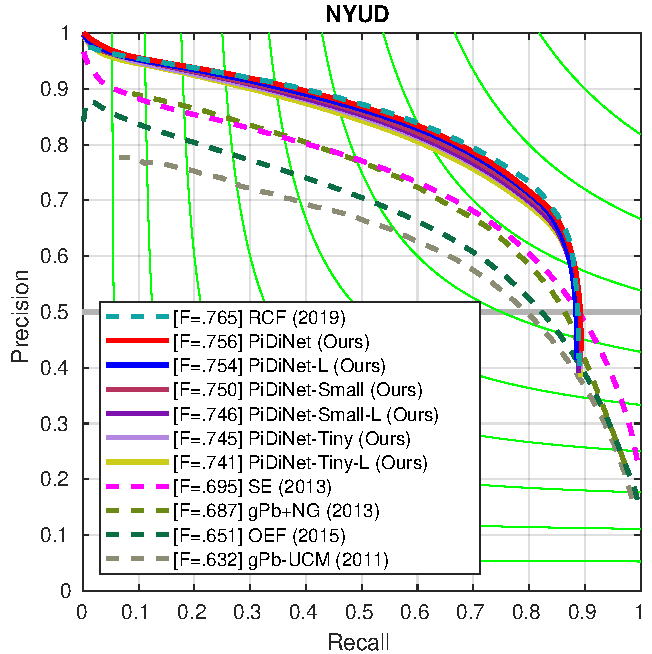
\includegraphics[width=0.9\linewidth]{images/nyud_pr2.pdf}
    \caption{Precision-Recall curves of our models and some competitors on NYUD dataset.}
    \label{fig:nyud_pr}
\end{figure}

\subsection{Precision-Recall Curves on NYUD Dataset}

The Precision-Reall curves of our methods and other approaches on NYUD dataset~\cite{shi2000nyud} are shown in Fig.~\ref{fig:nyud_pr}. The compared methods include RCF~\cite{liu2019richer}, SE~\cite{dollar2014se}, gPb+NG~\cite{gupta2013gpbng}, gPb-UCM~\cite{arbelaez2010bsds} and OEF~\cite{hallman2015oef}.

\begin{figure*}[t!]
    \centering
    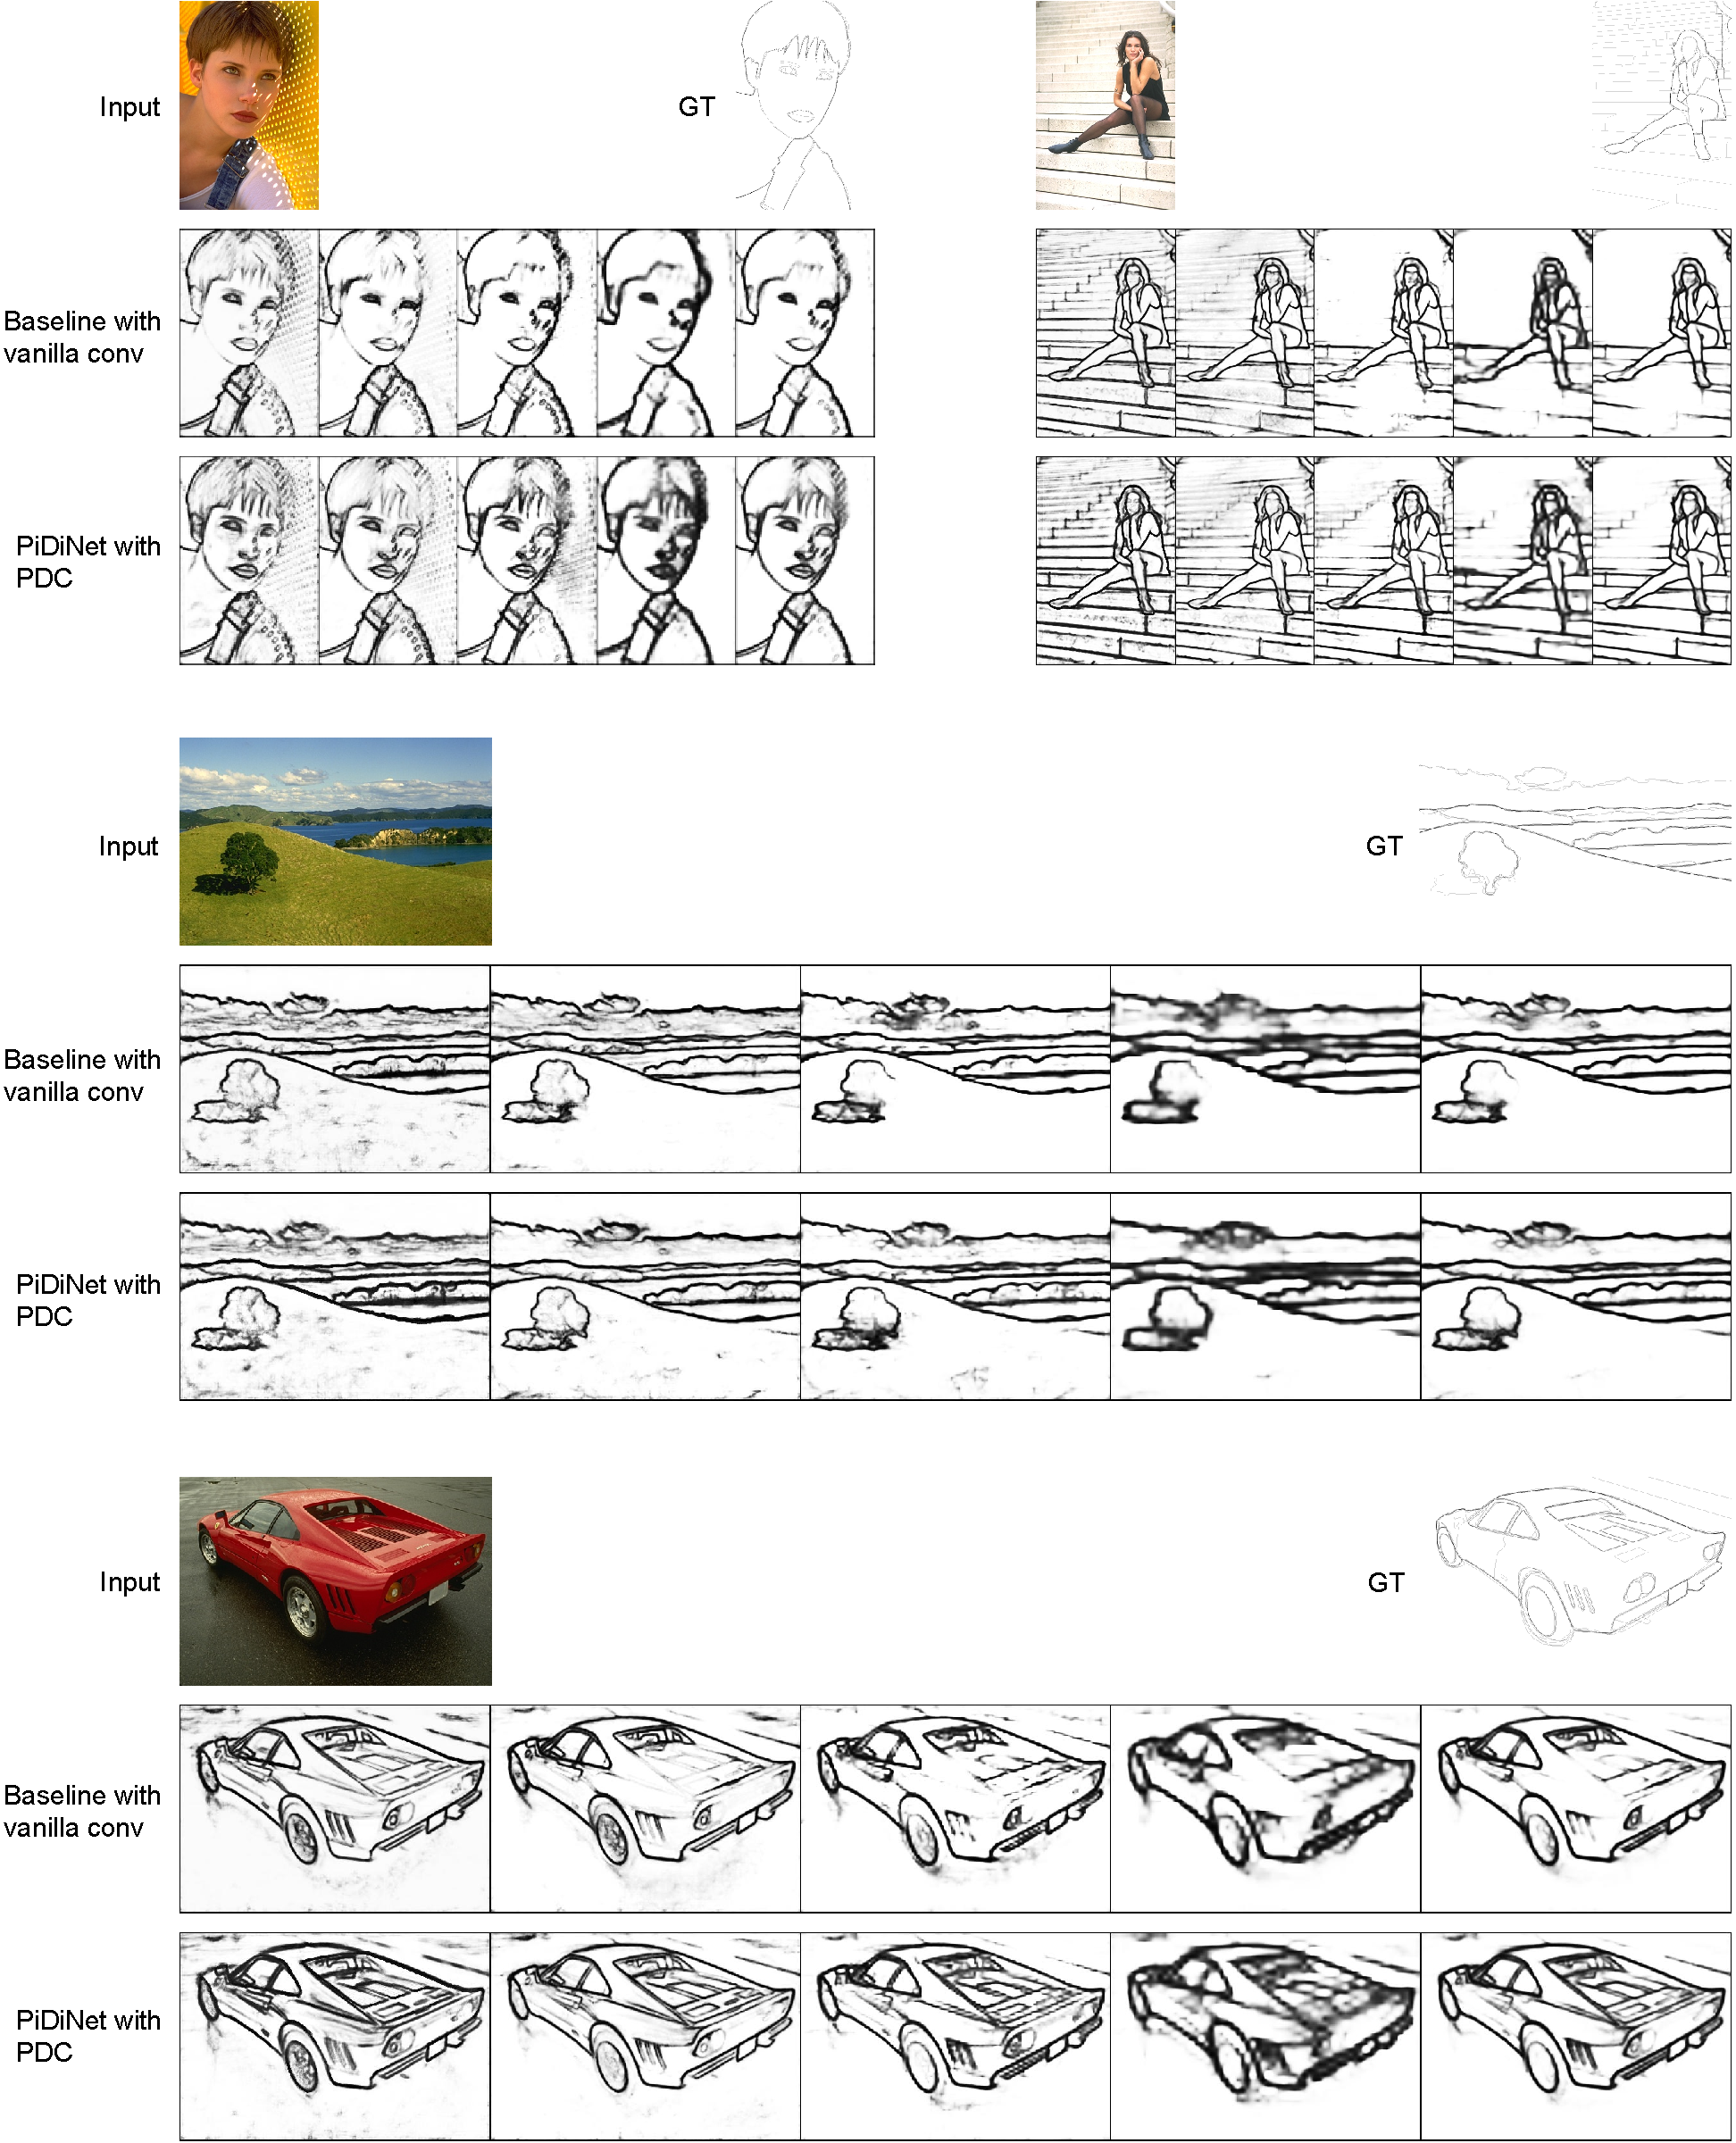
\includegraphics[width=0.97\linewidth]{images/supplement_fig1_cap.pdf}
    \caption{For each case, Top: input and ground truth image; Middle: edge maps from stage 1, 2, 3, 4 respectively and the final edge map, generated from the baseline architecture, Bottom: Corresponding edge maps generated from PiDiNet. Both the baseline architecture and PiDiNet were trained only using the BSDS500 dataset~\cite{arbelaez2010bsds}. Compared with the baseline, we can see that PiDiNet can detect more useful boundaries (\emph{e.g.}, bangs, stairs, the contour of the tree, the characteristic textures of the car).}
    \label{fig:stages}
\end{figure*}

\begin{figure*}[t!]
    \centering
    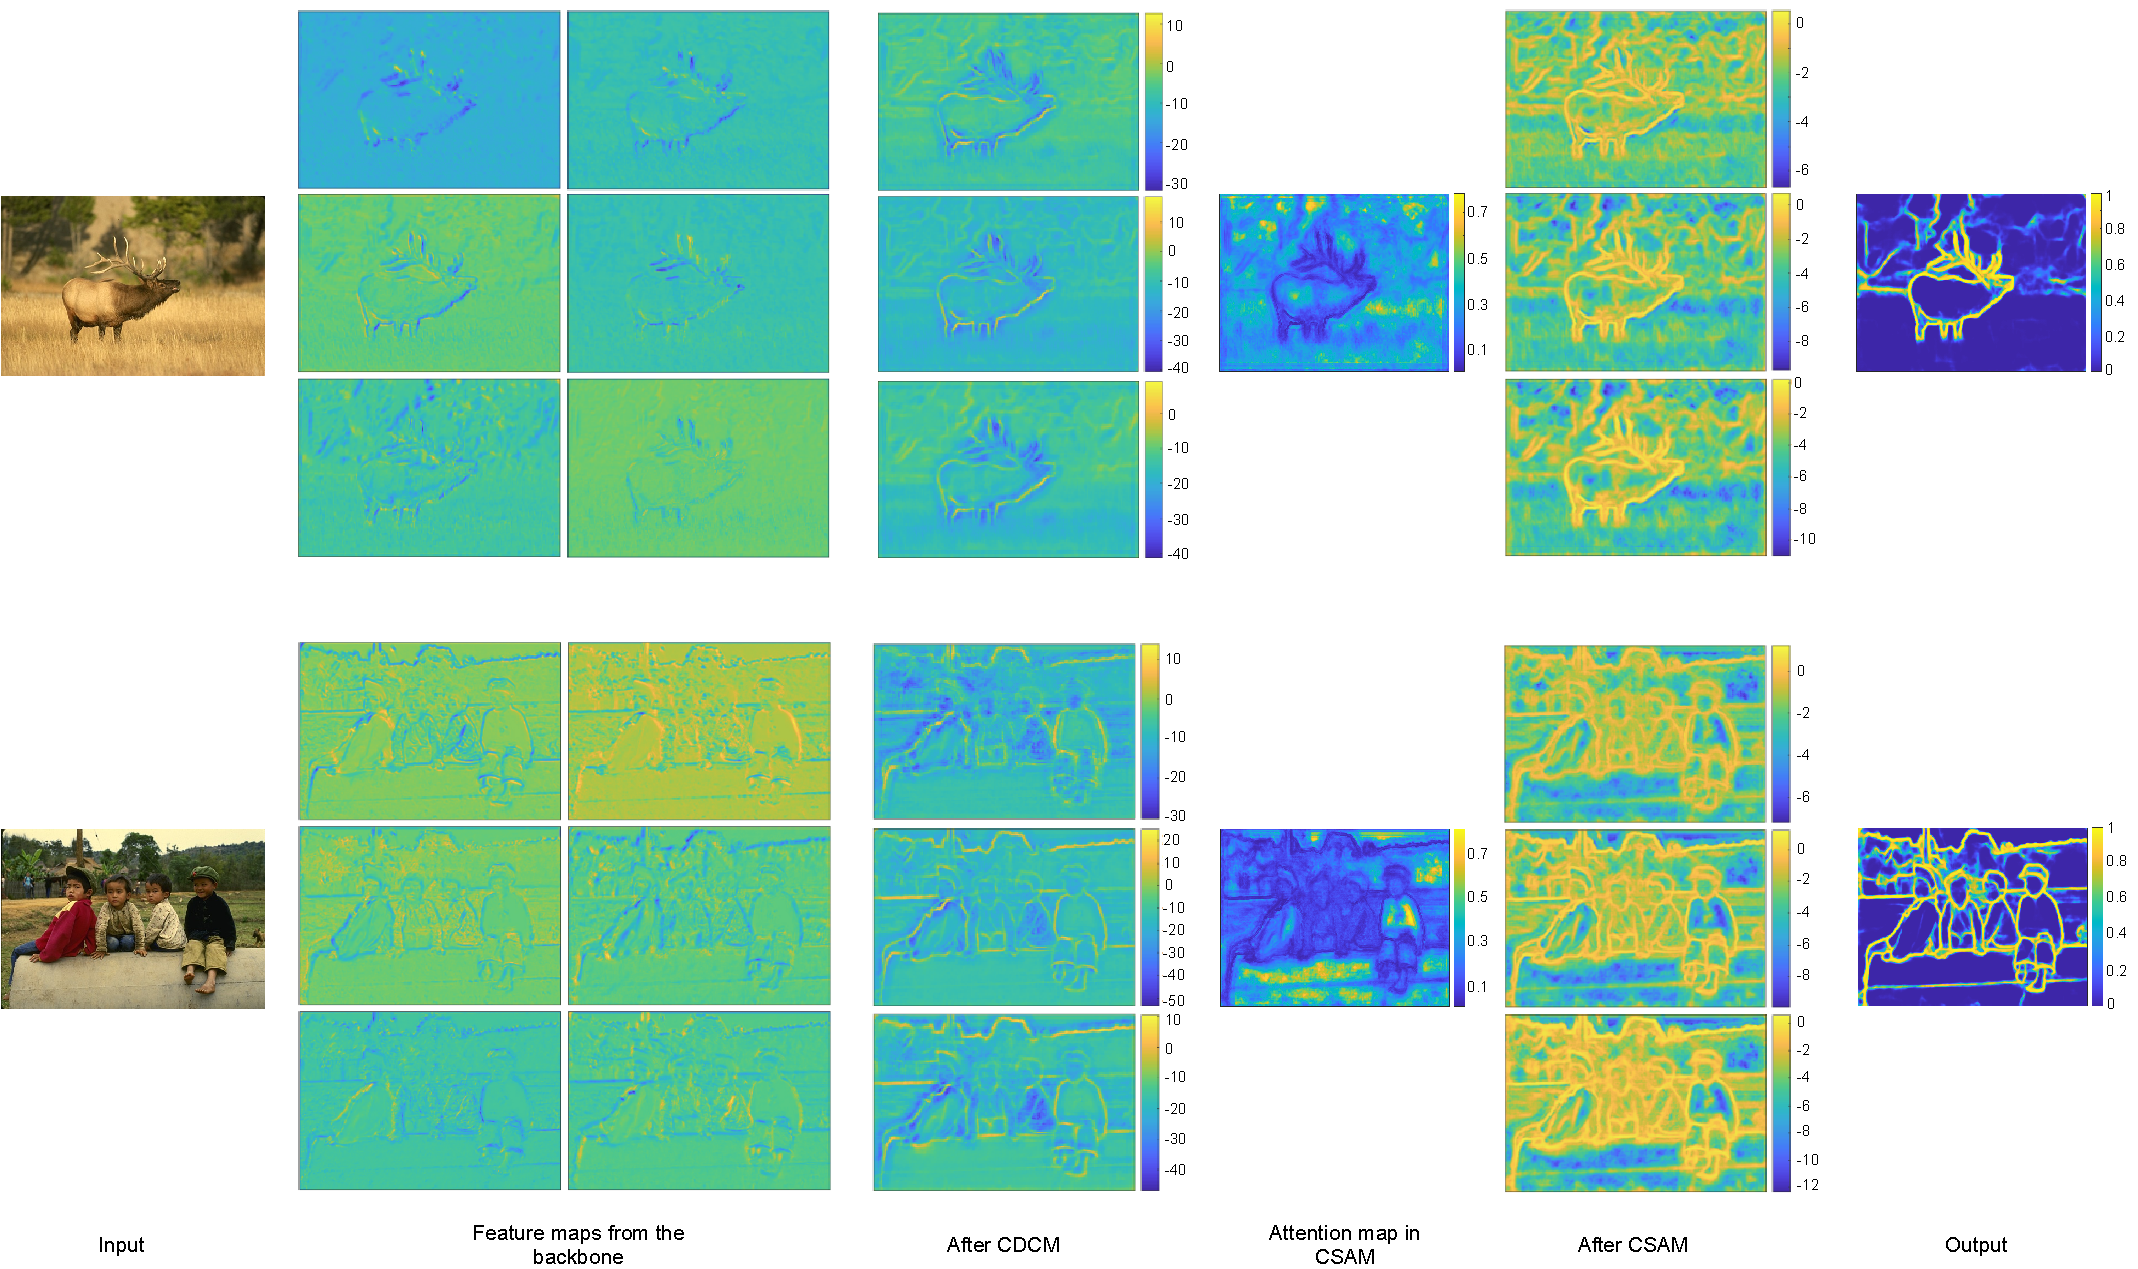
\includegraphics[width=1\linewidth]{images/supplement_fig_visual.pdf}
    \caption{CDCM and CSAM can further refine the feature maps with multi-scale feature extraction and the sample adaptive spatial attention mechanism. Note that in the attention maps generated by CSAM, pixels in the background show higher intensities. This makes sense as the background pixels after CDCM have negative values, hence they will be additionally suppressed through CSAM.}
    \label{fig:maps}
\end{figure*}

\subsection{Visualization}

\vspace{0.3em}
\noindent  \textbf{Edge Maps.} \quad The edge maps generated from the baseline architecture and PiDiNet are shown in Fig.~\ref{fig:stages}. Both models were trained using only the BSDS500 dataset without the mixed VOC dataset~\cite{mottaghi2014voc}. From the figure, it is proved that PDC can help PiDiNet effectively capture more useful boundaries, with the ability to extract rich gradient information that facilitates edge detection. 

\vspace{0.3em}
\noindent  \textbf{Intermediate Feature Maps.} \quad We also visualize the intermediate feature maps extracted from PiDiNet, to qualitatively demonstrate the effectiveness of the compact dilation convolution based module (CDCM) and the compact spatial attention module (CSAM), which are shown in Fig.~\ref{fig:maps}. It is concluded that both CDCM and CSAM take a positive role in PiDiNet on the edge detection task.


\end{document}
